\documentclass[../../main/main.tex]{subfiles}
\graphicspath{{./figures/}}

\setlength{\mtcindent}{-10pt}
\mtcsetoffset{minitoc}{-10pt}

\dominitoc
\faketableofcontents

\makeatletter
\renewcommand{\@chapapp}{\'Electrocin\'etique -- chapitre}
\makeatother

% \toggletrue{student}
% \HideSolutionstrue
\toggletrue{corrige}
\renewcommand{\mycol}{black}
% \renewcommand{\mycol}{gray}

\begin{document}
\setcounter{chapter}{5}

\chapter{Oscillateurs en r\'egime sinuso\"idal forc\'e}

\vfill

\begin{prgm}
	\begin{tcb}*(ror)"know"{Savoirs}
		\begin{itemize}[label=$\diamond$, leftmargin=10pt]
			\item Utiliser la représentation complexe pour étudier le régime forcé.
			\item Relier l’acuité d’une résonance au facteur de qualité.
		\end{itemize}
	\end{tcb}

	\begin{tcb}*(ror)"how"{Savoir-faire}
		\begin{itemize}[label=$\diamond$, leftmargin=10pt]
			\item Déterminer la pulsation propre et le facteur de qualité à partir de
			      graphes expérimentaux d’amplitude et de phase.
			\item Utiliser la représentation complexe pour étudier le régime forcé.
		\end{itemize}
	\end{tcb}
\end{prgm}

\vfill
\minitoc
\vfill

\newpage

\section{Introduction}
\subsection{Rappels oscillateurs}

Comme nous l'avions vu au chapitre 4, les oscillateurs amortis caractérisés par
une grandeur physique $x$ sont régis par une équation du type~:
\[ \xpp + \frac{\w_0}{Q} \xp + \w_0{}^2x = \w_0{}^2x\ind{eq}\]
Dans le cadre d'un signal d'entrée sinusoïdal $f(t) = A_0\cos(\wt)$ avec une
pulsation $\w$ (i.e. une fréquence $\w/2\pi$), cette équation devient
\[ \xpp + \frac{\w_0}{Q} \xp + \w_0{}^2x = \w_0{}^2f(t) = \w_0{}^2A_0\cos(\wt)\]
avec $A_0$ l'amplitude du forçage. \bigbreak

De la même manière qu'avec une excitation constante ($f(t) = E$ en échelon
montant), la solution de cette équation différentielle sera la somme d'une
solution homogène, caractéristique d'un régime transitoire, et d'une solution
particulière. On a vu que celle-ci prendrait la même forme que le signal
d'entrée, et sera donc également sinusoïdale. On a donc
\begin{gather*}
	x(t) = x_H(t) + x_P(t)\\
	\boxed{x_H(t) \xrightarrow[t\to+\infty]{} 0}
	\qet
	\boxed{x_P(t) = X\cos(\wt+\f)}
\end{gather*}

On rappelle que le régime sinusoïdal forcé correspond au régime où la solution
homogène est négligeable devant la solution particulière. On aura donc des
solutions de la forme suivante
\begin{center}
	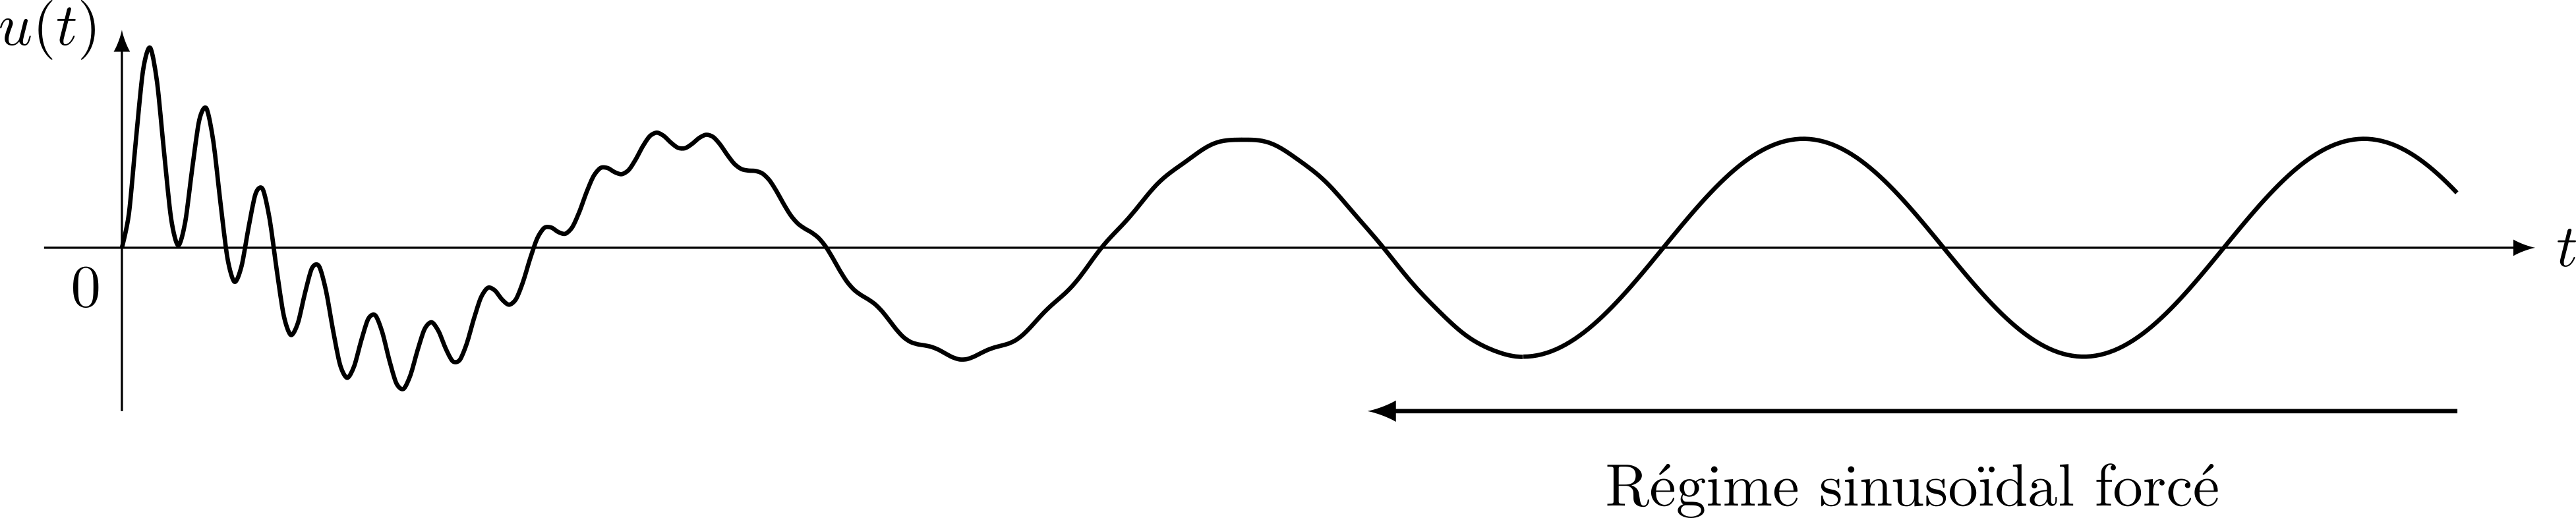
\includegraphics[width=\linewidth]{rsf_intro}
\end{center}
et le but de l'étude de ces systèmes en RSF est de trouver l'amplitude $X$ et la
phase $\f$.

\vspace{-10pt}
\subsection{Méthode des complexes}
Comme dans le chapitre précédent, le passage aux complexes permet d'exprimer
simplement les valeurs de $X$ et de $\f$. Pour passer en complexes, on note
\psw{
	\begin{gather*}
		\boxed{\xul{f}(t) = A_0\exr^{\jwt}}
		\qet
		\xul{x}(t) = X\exr^{\jj(\wt+\f)}
		\Lra
		\boxed{\xul{x}(t) = \xul{X}\exr^{\jwt}}
		\qavec
		\boxed{\xul{X} = X\exr^{\jj\f}}
	\end{gather*}
}
Ainsi, dériver en complexes revient à \textbf{multiplier par $\jj\w$}~: à partir
de l'équation différentielle d'un oscillateur, on aura alors, selon les
exemples, une amplitude de la forme
\psw{
	\[
		\boxed{
			\xul{X}
			= \frac{A_0}{1 + \jj Q \left( \frac{\w}{\w_r} - \frac{\w_r}{\w} \right)}
		}\]
}
\vspace{-15pt}

\begin{tcb}[cnt](impo){Attention}
	Cette forme de résonance n'est qu'un \textbf{exemple}. Elle dépend du
	système.
\end{tcb}

% \begin{gather*}
% 	\xpp + \frac{\w_0}{Q} \xp + \w_0{}^2x = \w_0{}^2f(t)
% 	\Lra
% 	\ddot{\xul{x}} + \frac{\w_0}{Q} \dot{\xul{x}} + \w_0{}^2\xul{x} = \w_0{}^2\xul{f}(t)\\
% 	\Lra
% 	(\jj\w)^2\xul{x} + \frac{\w_0}{Q}\jj\w\xul{x} + \w_0{}^2\xul{x} = \w_0{}^2\xul{f}(t)
% 	\Lra
% 	\left( \w_0{}^2-\w^2 + \jj \frac{\w\w_0}{Q} \right)
% 	\xul{X}\cancel{\exr^{\jwt}} = \w_0{}^2A_0\cancel{\exr^{\jwt}}\\
% 	\Lra
% 	\xul{X} = \frac{\w_0{}^2A_0}{ \w_0{}^2-\w^2 + \jj \frac{\w\w_0}{Q} }
% 	\Lra
% 	\xul{X} = \frac{A_0}
% 	{1 - \left(\dfrac{\w}{\w_0}\right)^2 + \jj \frac{\w}{Q\w_0}}
% \end{gather*}
On trouve donc l'amplitude du signal en en prenant le module~:
% \begin{gather*}
%     X
%         = \abs{\xul{X}}
%         = \frac{A_0}{
%             \sqrt{\left( 1 - \left(\dfrac{\w}{\w_0}\right)^2 \right)^2
%                 + \left(\dfrac{\w}{Q\w_0}\right)^2}}
% \end{gather*}

\psw{
	\[
		\boxed{
			X
			= \abs{\xul{X}}
			= \frac{A_0}{\sqrt{1 + Q^2\left( \frac{\w}{\w_r} - \frac{\w_r}{\w}
					\right)^2}}
		}
	\]
}
\vspace{-15pt}

\subsection{Notion de résonance et bande passante}
Par l'étude de l'amplitude, on retrouve bien que $X$ ne dépend pas des
conditions initiales, mais bien de l'amplitude d'entrée mais surtout
\textbf{dépend de la pulsation}. Notamment, on trouve que
\begin{gather*}
	\psw{
		\boxed{X \xrightarrow[\w\to+\infty]{} 0}
	}
	\qet
	\psw{
		\boxed{X \xrightarrow[\w\to0]{} 0}
	}
\end{gather*}

Ainsi, il y a une valeur particulière de pulsation telle que l'amplitude est
maximale~: c'est ce qu'on appelle la résonance.

\begin{tcb}[cnt, bld](defi){Résonance}
	\psw{
		Un oscillateur forcé présente une résonance si l’amplitude de ses
		oscillations est maximale pour une fréquence de forçage finie et non
		nulle. La fréquence correspondante est appelée fréquence de résonance.
	}
\end{tcb}

La représentation de l'amplitude en fonction de la pulsation est donc piquée
autour de son maximum $X_{\max}$ à la pulsation de résonance $\w_r$. Ce pic peut
être plus ou moins fin, ce que l'on caractérise par la \textbf{bande passante}
\begin{tcb}[sidebyside, righthand ratio=.4](defi){Bande passante}
	C'est le domaine de pulsations du forçage pour lequel
	\psw{
		\[
			\boxed{X(\w) > X_{\max}/\sqrt{2}}
		\]
	}
	\vspace{-15pt}
	\begin{itemize}
		\item \psw{
			      $\w_1$ et $\w_2$ les \textbf{pulsations de coupure}~;
		      }
		\item \psw{
			      $\D\w = \abs{\w_2 - \w_1}$ la \textbf{bande passante}~;
		      }
		\item \psw{
			      $\w_r/\D\w$ l'\textbf{acuité de la résonance}.
		      }
	\end{itemize}
	\tcblower
	\begin{center}
		\sswitch{
			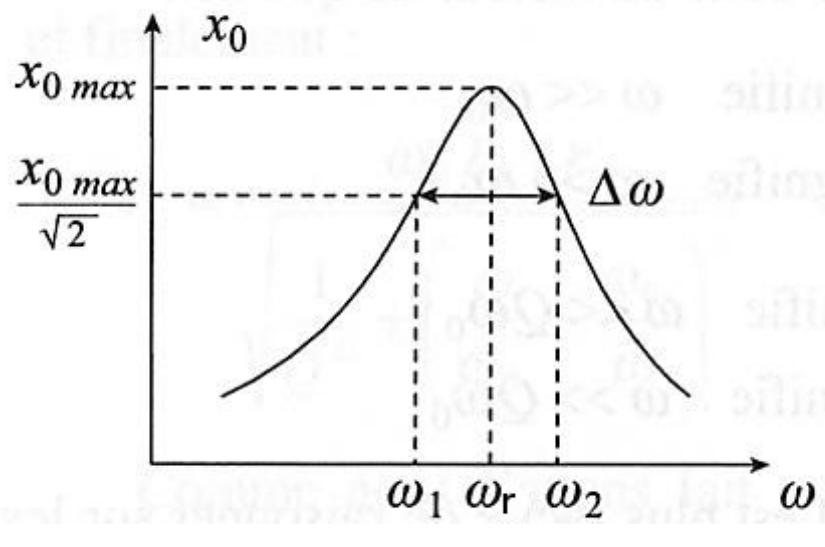
\includegraphics[width=\linewidth, draft=true]{bandepass_moche}
		}{
			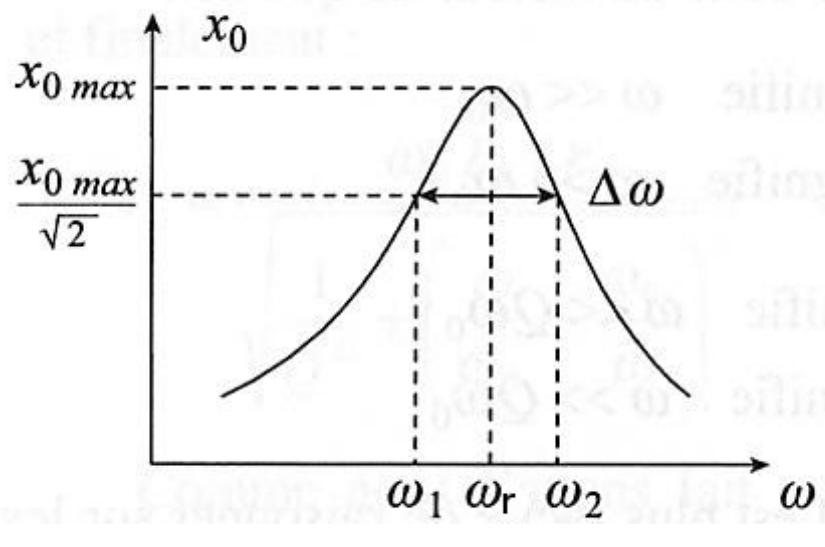
\includegraphics[width=\linewidth]{bandepass_moche}
		}
		\vspace{-15pt}
		\captionof{figure}{Bande passante et pic de résonance.}
	\end{center}
\end{tcb}

\section{Exemple d'oscillateur~: circuit RLC série en RSF}
\subsection{Présentation}

On étudie l'oscillateur amorti RLC série, dont le circuit en réel et en
complexes est le suivant~:
\begin{minipage}{\linewidth}
	\centering
	\sswitch{
		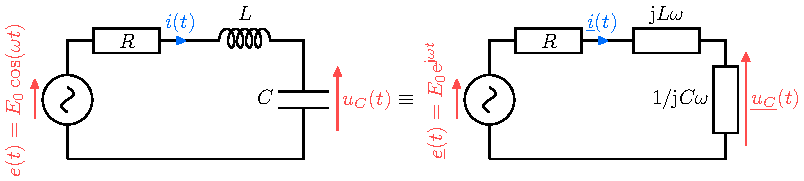
\includegraphics[width=.9\linewidth, draft=true]{rlc_sinu}
	}{
		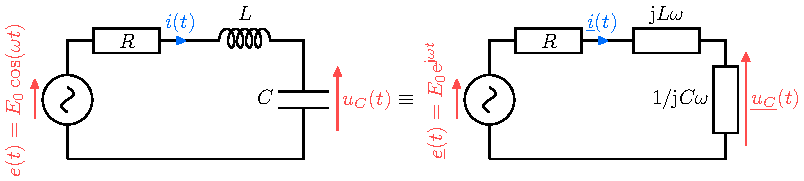
\includegraphics[width=.9\linewidth]{rlc_sinu}
	}
	\vspace{-15pt}
	\captionof{figure}{RLC série en RSF.}
\end{minipage}
% \begin{figure}[h!]
% 	\centering
% 	\sswitch{
% 		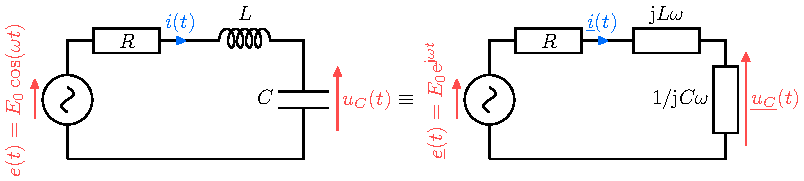
\includegraphics[width=.7\linewidth, draft=true]{rlc_sinu}
% 	}{
% 		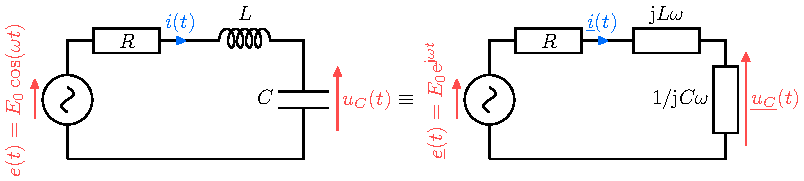
\includegraphics[width=.7\linewidth]{rlc_sinu}
% 	}
% 	\caption{RLC série en RSF.}
% 	\label{fig:rlc_sinu}
% \end{figure}

\begin{tcb}(rapp){Rappel}
	Pour un signal d'entrée $e(t) = E_0 \cos(\wt)$ les différentes tensions et
	intensités dans le circuit oscilleront \textbf{à la même pulsation $\w$}, et
	seront de la forme $u(t) = U\cos(\wt+\f_u) \qet i(t) = I\cos(\wt+\f_i)$ où
	$U,I$ et $\f_{u,i}$ sont quatre constantes dépendant du système et de
	l'excitation $\w$.
\end{tcb}

\subsection{Étude de l'intensité}
\begin{tcb}[sidebyside, righthand ratio=.3](defi)<lft>{Situation initiale}
	Pour étudier le comportement de l'intensité, on va comme d'habitude se
	ramener à une seule maille avec une impédance équivalente
	\[\Zu\ind{eq} = \Zu_R + \Zu_L + \Zu_C\]
	\tcblower
	\begin{center}
		\sswitch{
			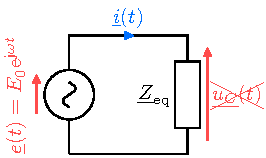
\includegraphics[width=\linewidth, draft=true]{rlc_zeq}
		}{
			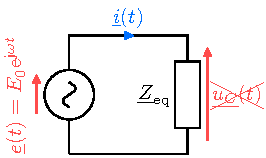
\includegraphics[width=\linewidth]{rlc_zeq}
		}
		\vspace{-15pt}
		\captionof{figure}{}
	\end{center}
\end{tcb}

\subsubsection{Équation}
\begin{tcb}(exem)<lft>{Développement}
	Avec l'impédance équivalente $\Zu\ind{eq}$, on a
	\psw{
		\begin{DispWithArrows*}
			E = \Zu\ind{eq}\Iu & =
			\left( R + \jlw + \frac{1}{\jcw} \right)\Iu
			\Arrow{On isole et on factorise par $\jj$}
			\\\Lra
			\Iu                    & =
			\frac{E}{R + \jj \left( L\w - \dfrac{1}{C\w} \right)}
			\Arrow{On factorise par $R$}
			\\\Lra
			\Iu                    & =
			\frac{E/R}{1 + \jj \left( \dfrac{L}{R}\w  - \dfrac{1}{RC\w}\right)}
		\end{DispWithArrows*}
	}
	\vspace{-15pt}
\end{tcb}
\begin{tcb}(tool)<lft>{Méthode de calcul}
	Ici on a factorisé par $R$ pour avoir un numérateur homogène à une intensité,
	et un dénominateur adimensionné. On aimerait aller plus loin, et transformer
	les $\frac{L}{R}$ et $RC$ en expressions semblables à $\w$, en les reliant à
	$\w_0 = \frac{1}{\sqrt{LC}}$. Pour cela, on se rappelle la forme canonique de
	l'équation différentielle sur $i(t)$ du RLC~:
	\[
		\dv[2]{i}{t} + \frac{R}{L} \dv{i}{t} + \frac{1}{LC}i = 0
		\Lra
		\dv[2]{i}{t} + \frac{\w_0}{Q} \dv{i}{t} + \w_0{}^2i = 0
	\]
	avec $\w_0$ la \textbf{pulsation propre} et $Q$ le \textbf{facteur de qualité},
	tels que
	\begin{gather*}
		\boxed{\w_0{}^2 = \frac{1}{LC}}
		\qet
		\frac{\w_0}{Q} = \frac{R}{L}
		\Lra
		\boxed{Q = \frac{1}{R} \sqrt{\frac{L}{C}}}
	\end{gather*}
	Ainsi,
	\psw{
		\begin{gather*}
			\boxed{\frac{L}{R} = \frac{Q}{\w_0}}
			\qet
			Q\w_0 = \frac{1}{R} \sqrt{\frac{\cancel{L}}{C}} \frac{1}{\sqrt{\cancel{L}C}}
			\Lra
			\boxed{ \frac{1}{RC} = Q\w_0}
		\end{gather*}
	}
\end{tcb}
\begin{tcb}(prop)<lft>{Résultat}
	On peut donc réécrire la fraction initiale~:
	\psw{
		\begin{gather*}
			\Iu = \frac{E/R}{1 + \jj \left( \dfrac{Q\w}{\w_0} - \dfrac{Q\w_0}{\w}
				\right)}
			\Lra
			\boxed{
				\Iu = \frac{E/R}{1 + \jj Q \left(
					\dfrac{\w}{\w_0} - \dfrac{\w_0}{\w}
					\right)}}
		\end{gather*}
	}
	\vspace{-15pt}
\end{tcb}

\subsubsection{Amplitude}

\begin{tcb}(prop)<lft>{Résultat}
	On trouve l'amplitude réelle en prenant le module, et comme en introduction
	cette amplitude dépend de la pulsation du système~:
	\psw{
		\[
			\boxed{
				I(\w)
				= \abs{\Iu}
				= \frac{E_0/R}{\sqrt{1 + Q^2\left( \dfrac{\w}{\w_0} - \dfrac{\w_0}{\w}
						\right)^2}}
			}
		\]
	}
	\vspace{-15pt}
\end{tcb}
\begin{tcb}(tool)<lft>{Méthode}
	On trouve le maximum de cette amplitude quand le dénominateur est minimal,
	c'est-à-dire
	\psw{
		\begin{gather*}
			I(\w_r) = I_{\max}
			\Lra
			1 + Q^2\left( \frac{\w_r}{\w_0} - \frac{\w_0}{\w_r} \right)^2 \text{minimal}\\
			\Lra
			Q^2\left( \frac{\w_r}{\w_0} - \frac{\w_0}{\w_r} \right)^2 = 0
			\Lra
			\boxed{\w_r = \w_0}
		\end{gather*}
	}
	\vspace{-15pt}
\end{tcb}
\begin{tcb}(ror){Conclusion}
	On trouve alors
	\psw{
		\[\boxed{
				I_{\max} = I(\w_0) = \frac{E_0}{R}
			}
			\qet
			\boxed{
				I\xrightarrow[\w\to0^+]{} 0}
			\qet
			\boxed{
				I\xrightarrow[\w\to+\infty]{} 0}
		\]
	}
	De ce résultat, nous observons qu'il \textbf{n'y a pas de condition pour avoir
		résonance en intensité}, et que \textbf{la pulsation de résonance est la
		pulsation propre du système}.
\end{tcb}

\vspace{-20pt}
\subsubsection{Phase}
\begin{tcb}(prop)<lft>{Résultat}
	Pour finir l'étude du système, il nous faut déterminer la phase en prenant
	l'argument de $\Iu$, en se souvenant que l'argument d'un rapport est la
	différence des arguments~:
	\psw{
		\begin{gather*}
			\f_i
			= \underbrace{\cancel{\arg*{E_0/R}}}_{=0}
			- \arg*{1 + \jj Q \left(
				\frac{\w}{\w_0} - \frac{\w_0}{\w}
				\right)}
			\\\Lra
			\boxed{\tan\f_i = -Q\left( \frac{\w}{\w_0} - \frac{\w_0}{\w} \right)}
			\qavec
			\boxed{\f_i \in \left] - \frac{\pi}{2}\,; \frac{\pi}{2} \right[}
		\end{gather*}
	}
	puisque $\cos\f_i > 0$ (la partie réelle est positive).
\end{tcb}
\begin{tcb}(ror){Conclusion}
	\psw{
		\[\tan\f_i \xrightarrow[\w\to0^+]{} +\infty \ra
			\boxed{\f_i \xrightarrow[\w\to0^+]{} +\pi/2}\]
		\[\tan(\f_i(\w_0)) = 0 \ra \boxed{\f_i(\w_0) = 0}\]
		\begin{center}
			\textbf{on peut détecter la résonance quand le déphasage entre
				$\iu$ et $\eu$ est nul.}
		\end{center}
		\[\tan\f_i \xrightarrow[\w\to+\infty]{} -\infty \ra
			\boxed{\f_i \xrightarrow[\w\to0^+]{} -\pi/2}\]
	}
\end{tcb}

\subsubsection{Facteur de qualité et bande passante}
\begin{tcb}(defi)<lft>{Définition}
	Nous avons déterminé l'amplitude et la phase du signal, ainsi que la
	pulsation de résonance. Pour finir de caractériser la résonance, il ne reste
	qu'à déterminer la bande passante. On cherche donc les pulsations de coupure
	telles que $I(\w) = \frac{I_{\max}}{\sqrt{2}}$.
\end{tcb}
\begin{tcb}(impl)<lft>{Implication}
	\psw{
		\begin{gather*}
			I(\w) = \frac{I_{\max}}{\sqrt{2}}
			\Lra
			\frac{E_0/R}{\sqrt{1 + Q^2\left( \frac{\w}{\w_0} - \frac{\w_0}{\w}
					\right)^2}}
			=
			\frac{E_0/R}{\sqrt{2}}
			\Lra
			\boxed{Q^2\left( \frac{\w}{\w_0} - \frac{\w_0}{\w} \right)^2 = 1}
		\end{gather*}
	}
\end{tcb}
\begin{tcb}(exem)<lft>{Calculs}
	On prend la racine carrée de cette équation, \textbf{en prenant les deux
		solutions possibles}~:
	\begin{DispWithArrows*}[format=LrL]
		&
		\psw{
			Q\left( \frac{\w}{\w_0} - \frac{\w_0}{\w} \right) = -1
		}
		& \qet
		\psw{
			Q\left( \frac{\w}{\w_0} - \frac{\w_0}{\w} \right) = 1
		}
		\CArrow{$\times \w\w_0$}
		\\\Lra
		&
		\psw{
			\left( \frac{\w}{\w_0} - \frac{\w_0}{\w} \right)\times \w\w_0 =
			- \frac{\w\w_0}{Q}
		}
		& \qet
		\psw{
			\left( \frac{\w}{\w_0} - \frac{\w_0}{\w} \right)\times \w\w_0 =
			\frac{\w\w_0}{Q}
		}
		\Arrow{On développe}
		\\\Lra
		&
		\psw{
			\w^2 - \w_0{}^2 = -\frac{\w\w_0}{Q}
		}
		& \qet
		\psw{
			\w^2 - \w_0{}^2 = \frac{\w\w_0}{Q}
		}
		\Arrow{Trinôme}
		\\\Lra
		&
		\psw{
			\boxed{ \w^2 + \frac{\w_0}{Q}\w - \w_0{}^2 = 0}
		}
		& \qet
		\psw{
			\boxed{ \w^2 - \frac{\w_0}{Q}\w - \w_0{}^2 = 0}
		}
		\Arrow{Discriminant}
		\\\Ra
		&
		\psw{
			\Delta =
			\frac{\w_0{}^2}{Q} + 4\w_0{}^2
		}
		& \psw{\quad \Lra \quad}
		\psw{
			\Delta =
			\frac{\w_0{}^2}{Q^2} \left( 1 + 4Q^2 \right)
		}
		\Arrow{Solutions}
		\\\Ra
		&
		\psw{
			\w_{1,\pm} = -\frac{\w_0}{2Q} \pm \frac{\w_0}{2Q} \sqrt{1+4Q^2}
		}
		& \qet
		\psw{
			\w_{2,\pm} = \frac{\w_0}{2Q} \pm \frac{\w_0}{2Q} \sqrt{1+4Q^2}
		}
		\Arrow{Factorisation}
		\\\Lra
		&
		\psw{
			\w_{1,\pm} = \frac{\w_0}{2Q} \left(-1 \pm \sqrt{1+4Q^2}\right)
		}
		& \qet
		\psw{
			\w_{2,\pm} = \frac{\w_0}{2Q} \left(1 \pm \sqrt{1+4Q^2}\right)
		}
	\end{DispWithArrows*}
	De ces quatre racines, seules deux sont positives~: la solution avec $-1 -
		\sqrt{1+4Q^2}$ est évidemment négative, et celle avec $1 - \sqrt{1+4Q^2}$
	également. Ainsi, il ne nous reste que
	\psw{
		\begin{gather*}
			\boxed{
				\w_{1,+} = \frac{\w_0}{2Q} \left( \sqrt{1+4Q^2}-1 \right)
				\qet
				\w_{2,+} = \frac{\w_0}{2Q} \left( \sqrt{1+4Q^2}+1 \right)
			}
		\end{gather*}
	}
\end{tcb}

\begin{tcb}(prop)<lft>{Résultat}
	Il ne reste qu'à calculer la différence pour avoir la bande passante~:
	\psw{
		\begin{gather*}
			\boxed{\D\w = \w_2 - \w_1 = \frac{\w_0}{Q}
				\Lra
				Q = \frac{\w_0}{\D\w}
			}
		\end{gather*}
	}
	ce qui est également une \textbf{nouvelle définition de $Q$}~! En effet, cette
	égalité traduit le fait qu'à haut facteur de qualité, la bande passante est
	très faible, ou que \textbf{l'acuité de la résonance est élevée}.
\end{tcb}

\begin{center}
	\sswitch{
		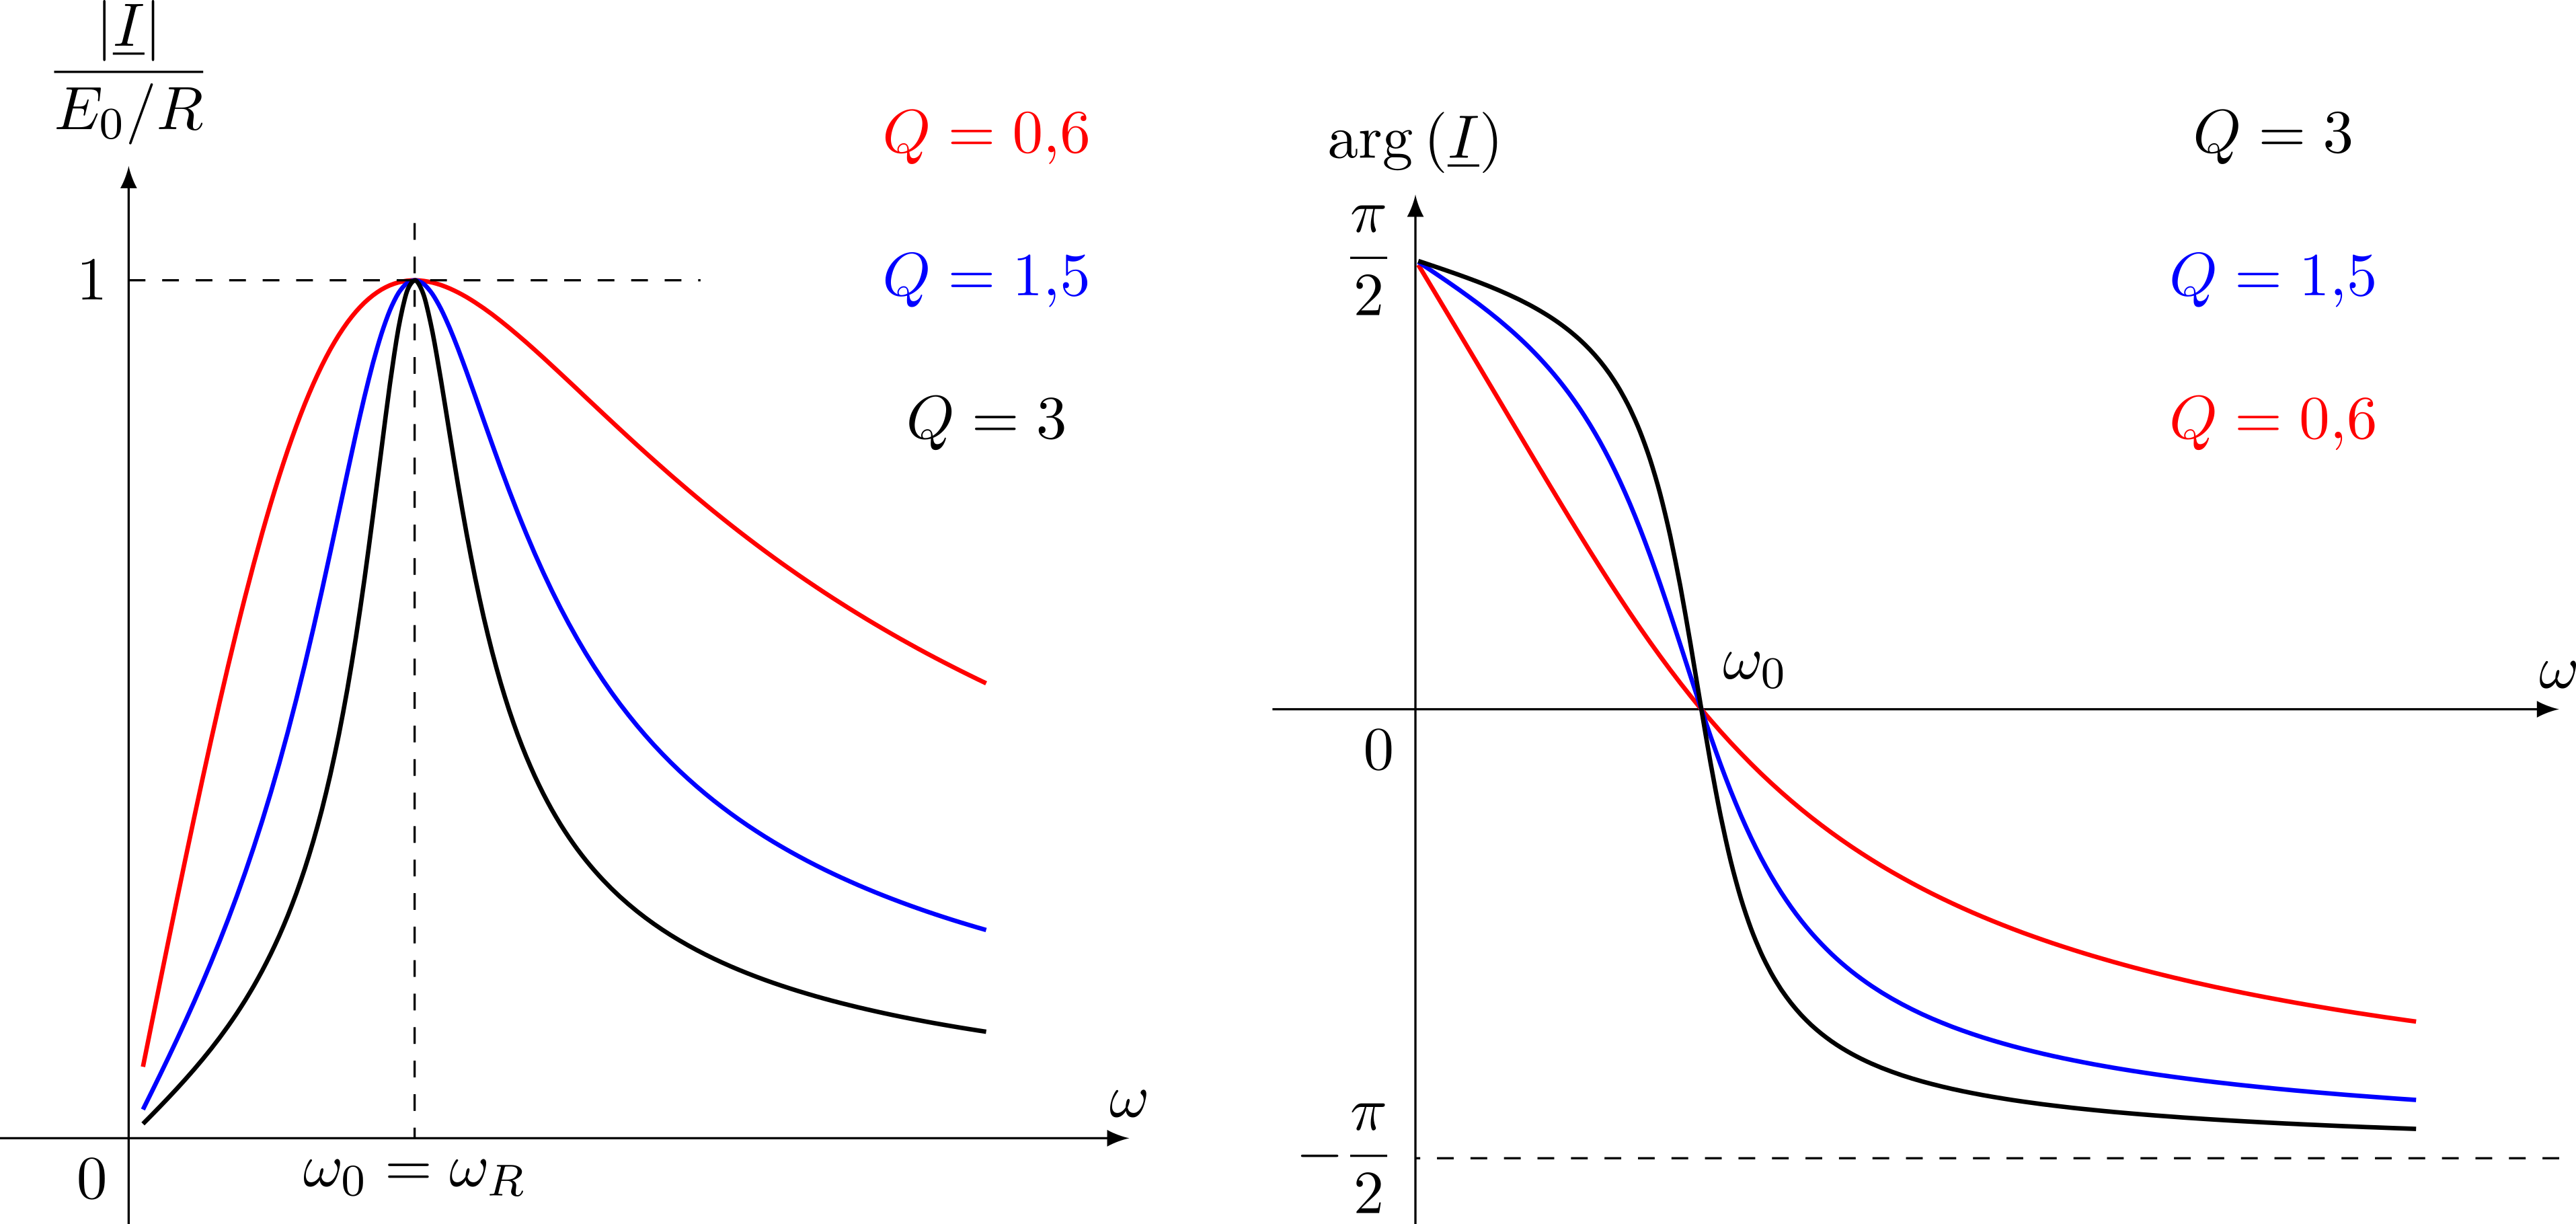
\includegraphics[width=.8\linewidth, draft=true]{rlc_i-ampphase}
	}{
		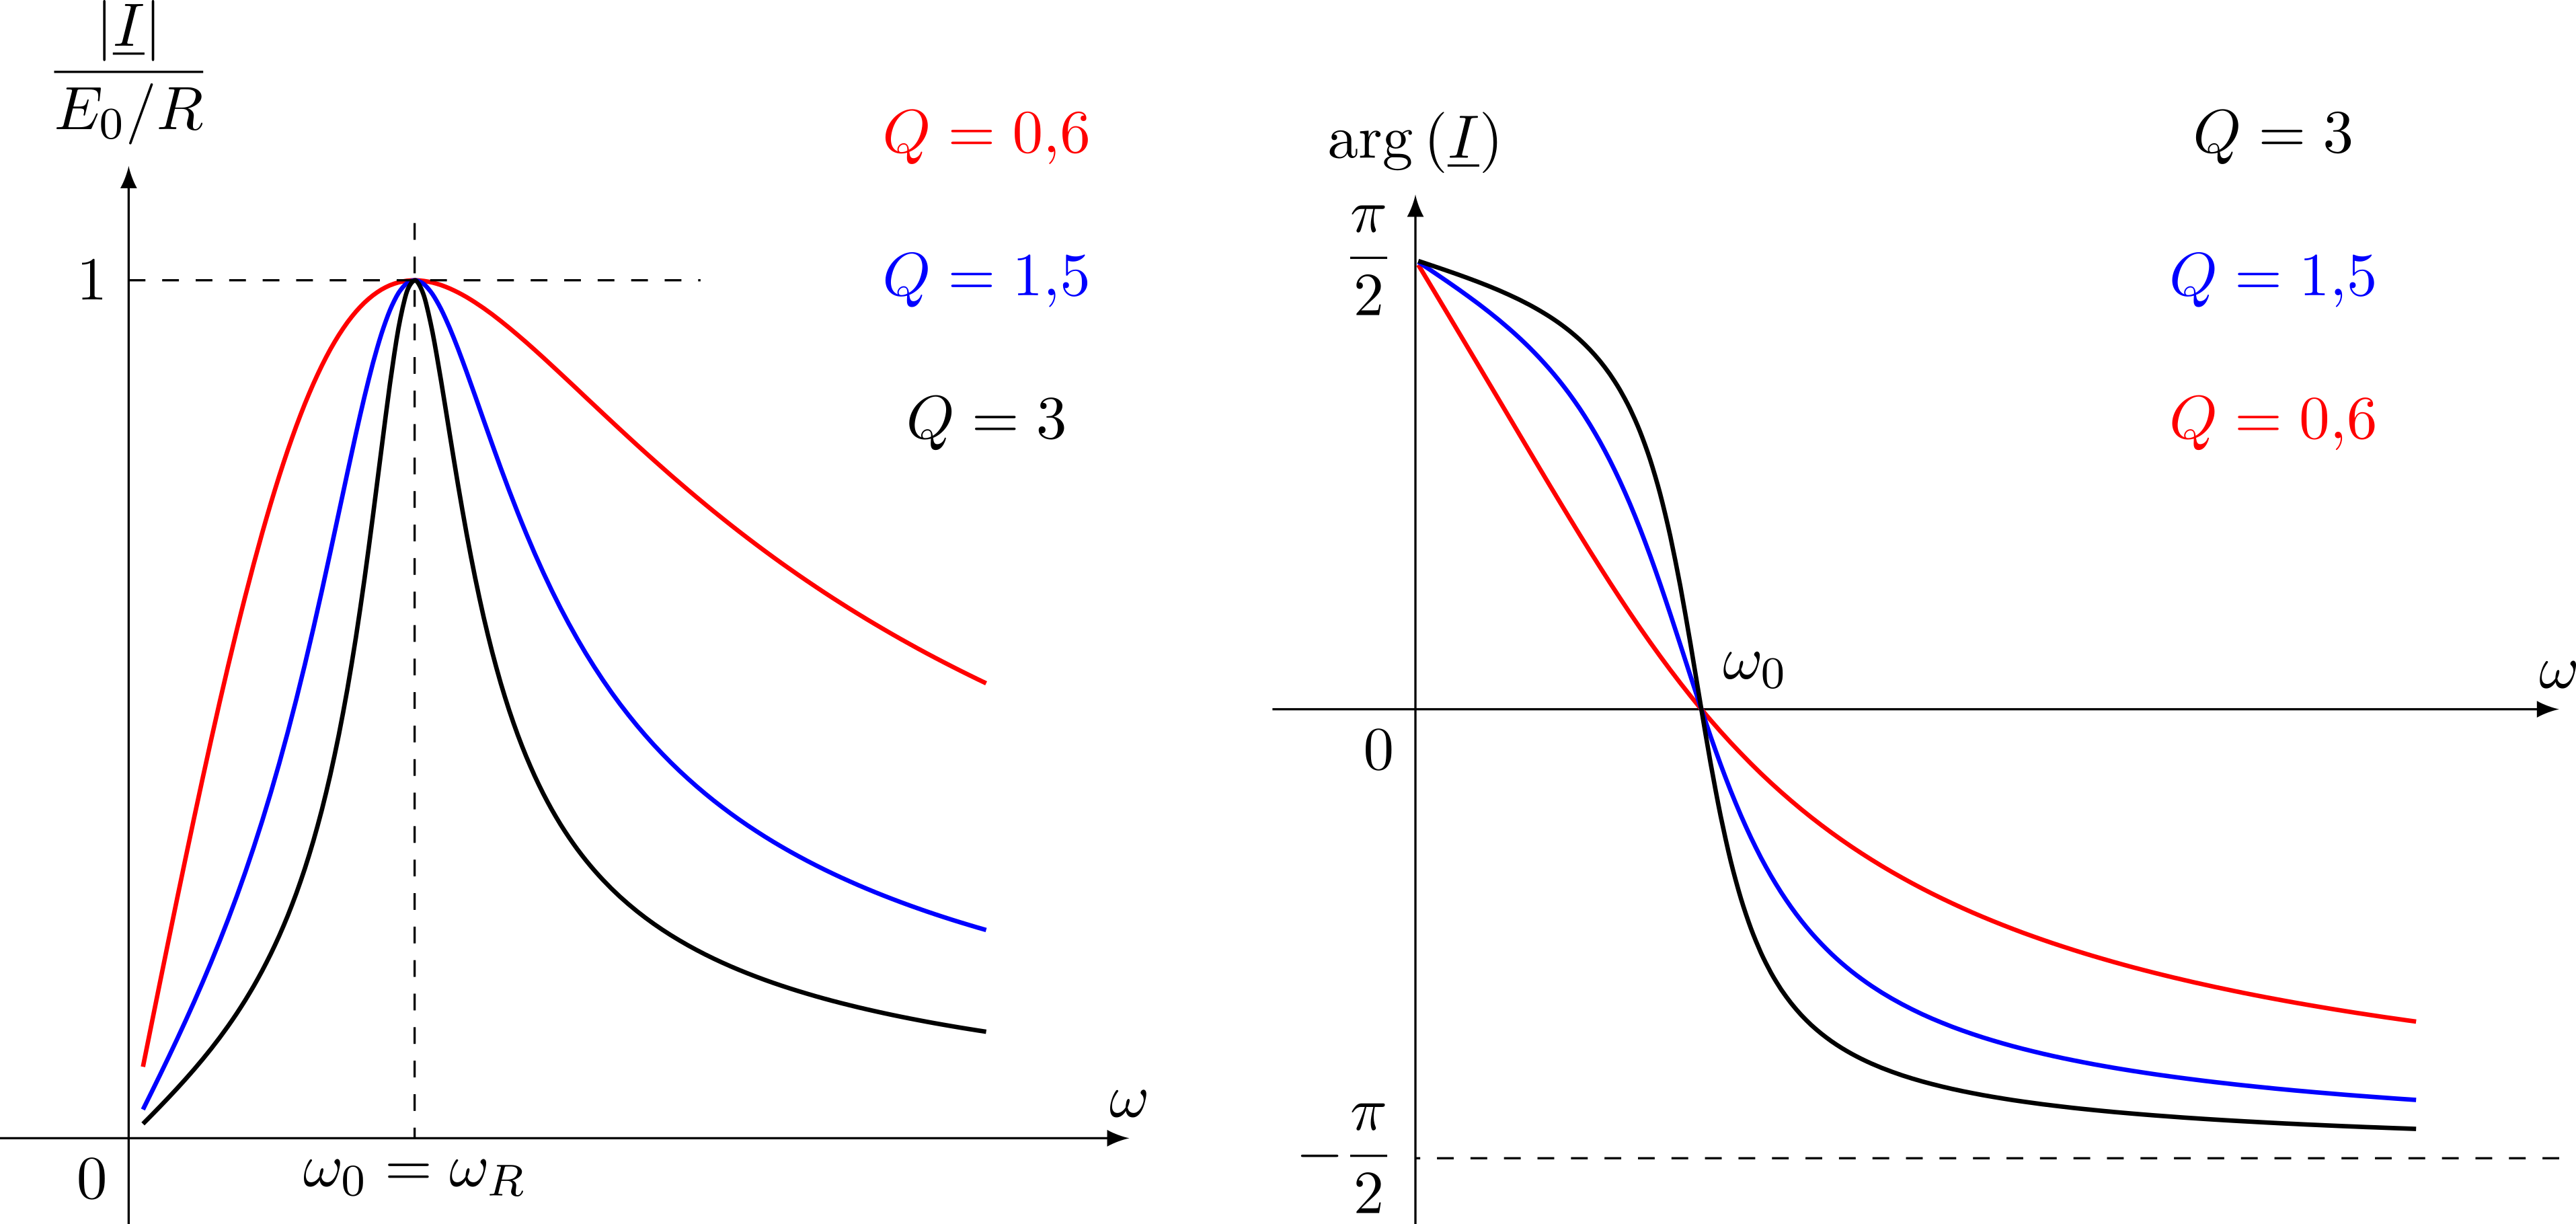
\includegraphics[width=.8\linewidth]{rlc_i-ampphase}
	}
	\captionof{figure}{Amplitude et phase en fonction de $Q$ pour $\Iu$ en RLC
		série.}
\end{center}

\subsection{Étude de la tension}
On repart du circuit en complexes, avec $\xul{u_C}(t) = \Uu\exr^{\jwt}$ et
$\eu(t) = E\exr^{\jwt}$, et on applique le pont diviseur de tension.

\subsubsection{Amplitude complexe}
\begin{tcb}(defi)<lft>{Situation initiale}
	\vspace{-20pt}
	\begin{minipage}{0.40\linewidth}
		\begin{center}
			\sswitch{
				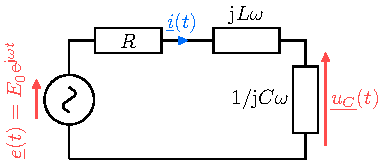
\includegraphics[width=\linewidth, draft=true]{rlc_u-circ}
			}{
				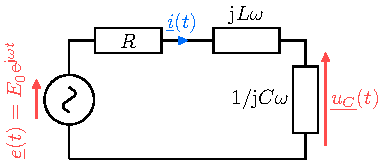
\includegraphics[width=\linewidth]{rlc_u-circ}
			}
			\vspace{-15pt}
			\captionof{figure}{RLC série~: étude de $\uu_C$.}
		\end{center}
	\end{minipage}
	\hfill
	\begin{minipage}{0.60\linewidth}
		\begin{tcb}(prop)<rgt>'r'{Résultat}
			\psw{
				\begin{DispWithArrows*}
					\Uu &= \frac{1/\jcw}{R + \jlw + 1/\jcw}E
					\CArrow{$\times \jcw$}
					\\\Lra
					\Uu &= \frac{E}{1 - (LC\w)^2 + \jj RC\w}
					\Arrow{$\w_0$ et $Q$}
					\\\Lra
					\Aboxed{
						\Uu &=
						\frac{E}{1 -
							\left( \dfrac{\w}{\w_0} \right)^2 +
							\jj\dfrac{\w}{Q\w_0}}
					}
				\end{DispWithArrows*}
			}
			\vspace{-15pt}
		\end{tcb}
	\end{minipage}
\end{tcb}
\begin{tcb}(tool)<lft>{Méthode de calcul}
	Ici encore, on a factorisé par $1/\jcw$ pour avoir un numérateur homogène
	à une tension et
	un dénominateur adimensionné d'abord. Ensuite puis pour aller plus loin, on
	transformer les $LC$ et $RC$ en expressions semblables à $\w$, en les
	reliant à $\w_0$. On a comme précédemment
	\psw{
		\begin{gather*}
			\boxed{\w_0{}^2 = \frac{1}{LC}}
			\qet
			\boxed{Q = \frac{1}{R} \sqrt{\frac{L}{C}}}
			\qdonc
			Q\w_0 = \frac{1}{R} \sqrt{\frac{\cancel{L}}{C}} \frac{1}{\sqrt{\cancel{L}C}}
			\Lra
			\boxed{ \frac{1}{RC} = Q\w_0}
		\end{gather*}
	}
\end{tcb}

\subsubsection{Amplitude réelle et condition de résonance}
\begin{tcb}(prop)<lft>{Résultat}
	On trouve l'amplitude réelle en prenant le module, et comme en introduction
	cette amplitude dépend de la pulsation du système~:
	\psw{
		\[
			\boxed{
				U(\w)
				= \abs{\Uu}
				= \frac{E_0}{
					\sqrt{\left( 1 - \left(\dfrac{\w}{\w_0}\right)^2 \right)^2
						+ \left(\dfrac{\w}{Q\w_0}\right)^2}}
			}
		\]
	}
\end{tcb}
\begin{tcb}(tool)<lft>{Méthode}
	On trouve le maximum de cette amplitude quand le dénominateur est
	\textbf{non nul} et minimal, c'est-à-dire
	\psw{
		\begin{gather*}
			U(\w_r) = U_{\max}
			\Lra
			\left( 1 - \left(\dfrac{\w}{\w_0}\right)^2 \right)^2
			+ \left(\dfrac{\w}{Q\w_0}\right)^2 \text{minimal}
		\end{gather*}
	}
	Soit $X = \left( \dfrac{\w}{\w_0} \right)^2$, et $f(X) = \left(1 - X\right)^2
		+ \dfrac{X}{Q^2}$, la fonction que l'on cherche à minimiser~: on cherche donc
	quand est-ce que sa dérivée est nulle, c'est-à-dire
	\psw{
		\begin{DispWithArrows*}
			f'(X_r) &= 0
			\Arrow{On dérive}
			\\\Lra
			-2 \left( 1-X_r \right) + \frac{1}{Q^2} &= 0
			\Arrow{On isole}
			\\\Lra
			X_r-1 = - \frac{1}{2Q^2}
			& \Lra
			X_r = 1 - \frac{1}{2Q^2}
			\Arrow{$X_r = \left( \frac{\w_r}{\w_0} \right)^{2}$}
			\\\Lra
			\w_r = \w_0 \sqrt{1 - \frac{1}{2Q^2}}
			& \Lra
			\boxed{
				\w_r = \frac{\w_0}{Q} \sqrt{Q^{2} - \frac{1}{2}}
			}
		\end{DispWithArrows*}
	}
	\vspace{-15pt}
	ce qui n'est défini \textbf{que si} $Q > \dfrac{1}{\sqrt{2}}$. On calcule
	alors $f(X_r)$ en injectant la solution~:
	\psw{
		\begin{DispWithArrows*}[]
			f(X_r) &=
			\left( \cancel{1} -
			\left( \cancel{1} - \frac{1}{2Q^{2}} \right)
			\right)^{2} +
			\frac{1}{Q^{2}} \left( 1 - \frac{1}{2Q^{2}} \right)
			\Arrow{On simplifie et développe}
			\\\Lra
			f(X_r) &=
			\left( \frac{1}{2Q^{2}} \right)^{2} + \frac{1}{Q^{2}} - \frac{1}{2Q^{4}}
			\Arrow{Même denominateur}
			\\\Lra
			f(X_r) &=
			\frac{1}{4Q^{2}} - \frac{2}{4Q^{4}} + \frac{1}{Q^{2}}
			\Arrow{On calcule}
			\\\Lra
			f(X_r) &=
			\frac{1}{Q^{2}} - \frac{1}{4Q^{4}}
			\Arrow{On factorise}
			\\\Lra
			\Aboxed{
				f(X_r) &=
				\frac{1}{Q^{2}}\left( 1 - \frac{1}{4Q^{2}} \right)}
			% \frac{1}{4Q^{4}}\left( 4Q^{2} - 1 \right)
		\end{DispWithArrows*}
	}
	\vspace{-15pt}
\end{tcb}
\begin{tcb}[breakable](ror){Conclusion}
	On trouve alors~:
	\begin{itemize}[leftmargin=60pt]
		\item[$\mathbf{Q \leq 1/\sqrt{2}}$] :
		      \psw{
			      \textbf{pas de résonance}, l'amplitude est maximale pour
			      \[\boxed{\w = 0 \qet U(0) = E_0}\]
		      }
		      \vspace{-15pt}
		\item[$\mathbf{Q > 1/\sqrt{2}}$] :
		      \psw{
			      La résonance existe, l'amplitude est maximale pour
			      \[
				      \boxed{\w_r = \frac{\w_0}{Q} \sqrt{Q^{2} - \frac{1}{2}} < \w_0}
				      \qet
				      \boxed{U(\w_r) = \frac{QE}{\sqrt{1 - \frac{1}{4Q^{2}}}}}
			      \]
		      }
		\item[$\mathbf{Q > 5}$] :
		      \psw{
			      \[
				      \boxed{\w_r \approx \w_0}
				      \qet
				      \boxed{U(\w_r) \approx QE}
			      \]
		      }
		      \vspace{-15pt}
	\end{itemize}
	De ce résultat, nous observons qu'il \textbf{n'y a pas toujours résonance en
		tension}, et que \textbf{la résonance est d'autant aiguë que $\mathbf{Q}$
		est élevé}.
\end{tcb}

\subsubsection{Phase}
\begin{tcb}(prop)<lft>{Résultat}
	Ici aussi, on détermine la phase en prenant l'argument de l'amplitude
	complexe~:
	\psw{
		\begin{align*}
			\f_u     & = \underbrace{\cancel{\arg*{E_0}}}_{=0}
			- \arg*{ 1 - \left(\frac{\w}{\w_0}\right)^2 + \jj \frac{\w}{Q\w_0}}
			\\\Lra
			\Aboxed{
			\tan\f_u & = -\frac{\w}{Q\w_0\left(
					1 - \left( \frac{\w}{\w_0}
					\right)^2\right)}
			}
			\qavec
			\boxed{
			\f_u \in \left] -\pi\,; 0 \right[}
		\end{align*}
	}
\end{tcb}
\begin{tcb}(ror){Conclusion}
	\vspace{-15pt}
	\psw{
		\begin{align*}
			\tan\f_u \xrightarrow[\w\to0^+]{} 0
			\Ra &
			\boxed{\f_u \xrightarrow[\w\to0^+]{} 0}
			\\
			\tan(\f_u(\w_0)) \longrightarrow -\infty
			\Ra &
			\boxed{\f_u(\w_0) = - \frac{\pi}{2}}
			\\
			\tan\f_u \xrightarrow[\w\to+\infty]{} 0
			\Ra &
			\boxed{\f_u \xrightarrow[\w\to0^+]{} - \pi}
		\end{align*}
	}
	\vspace{-15pt}
\end{tcb}

\begin{minipage}{\linewidth}
	\centering
	\sswitch{
		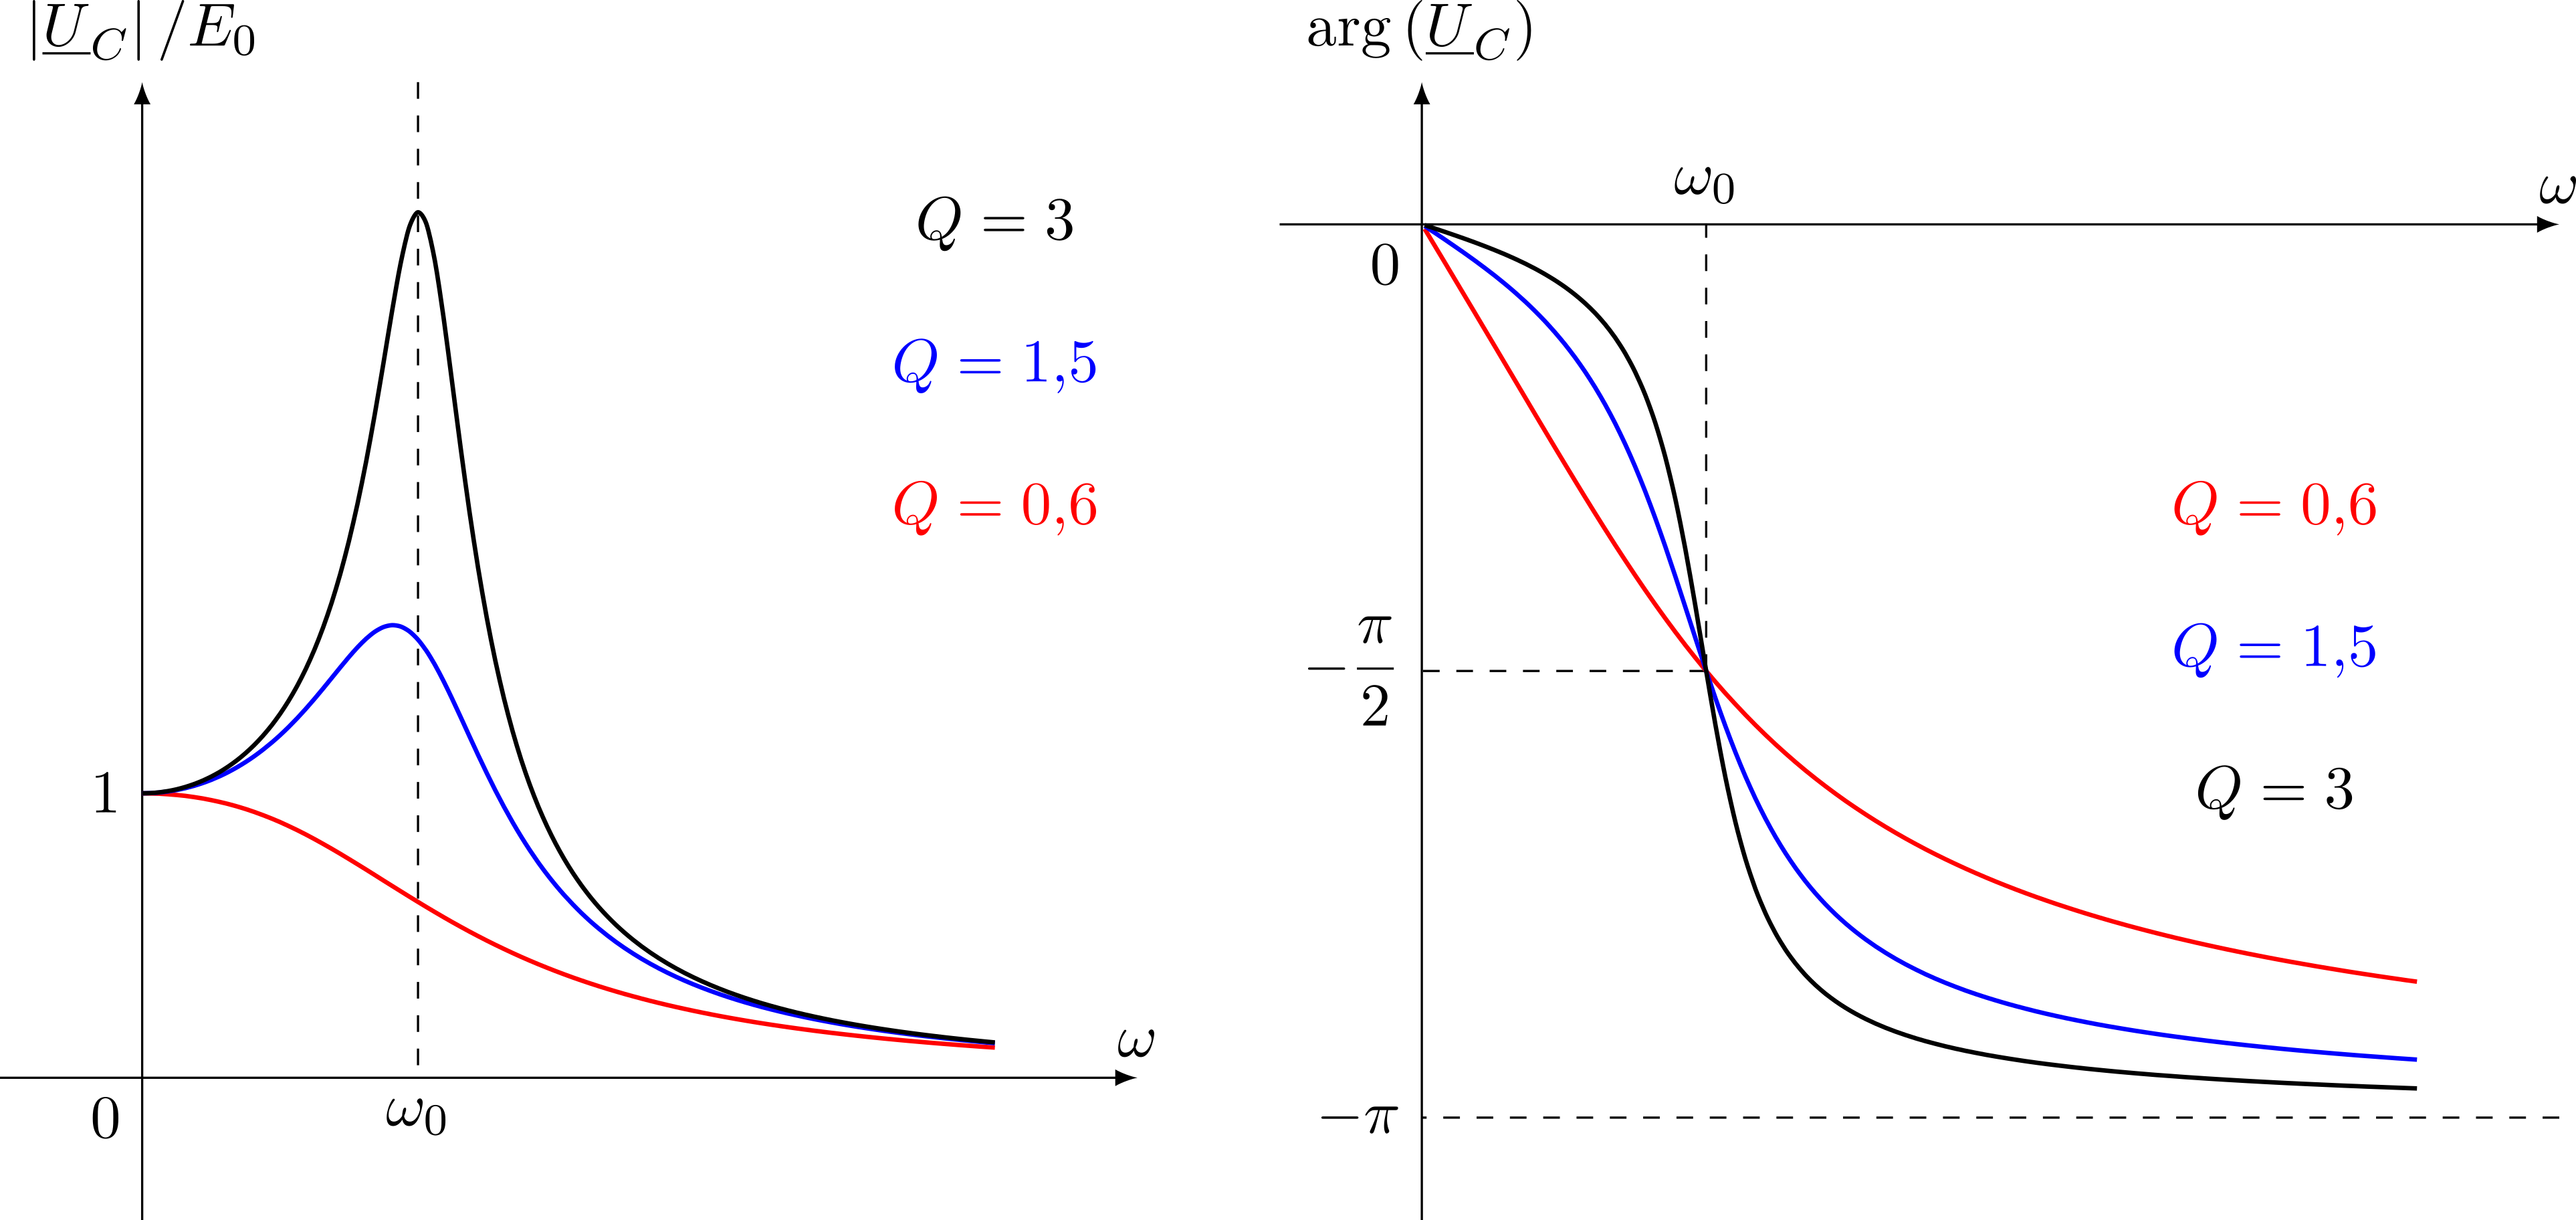
\includegraphics[width=0.9\linewidth, draft=true]{rlc_u-ampphase}
	}{
		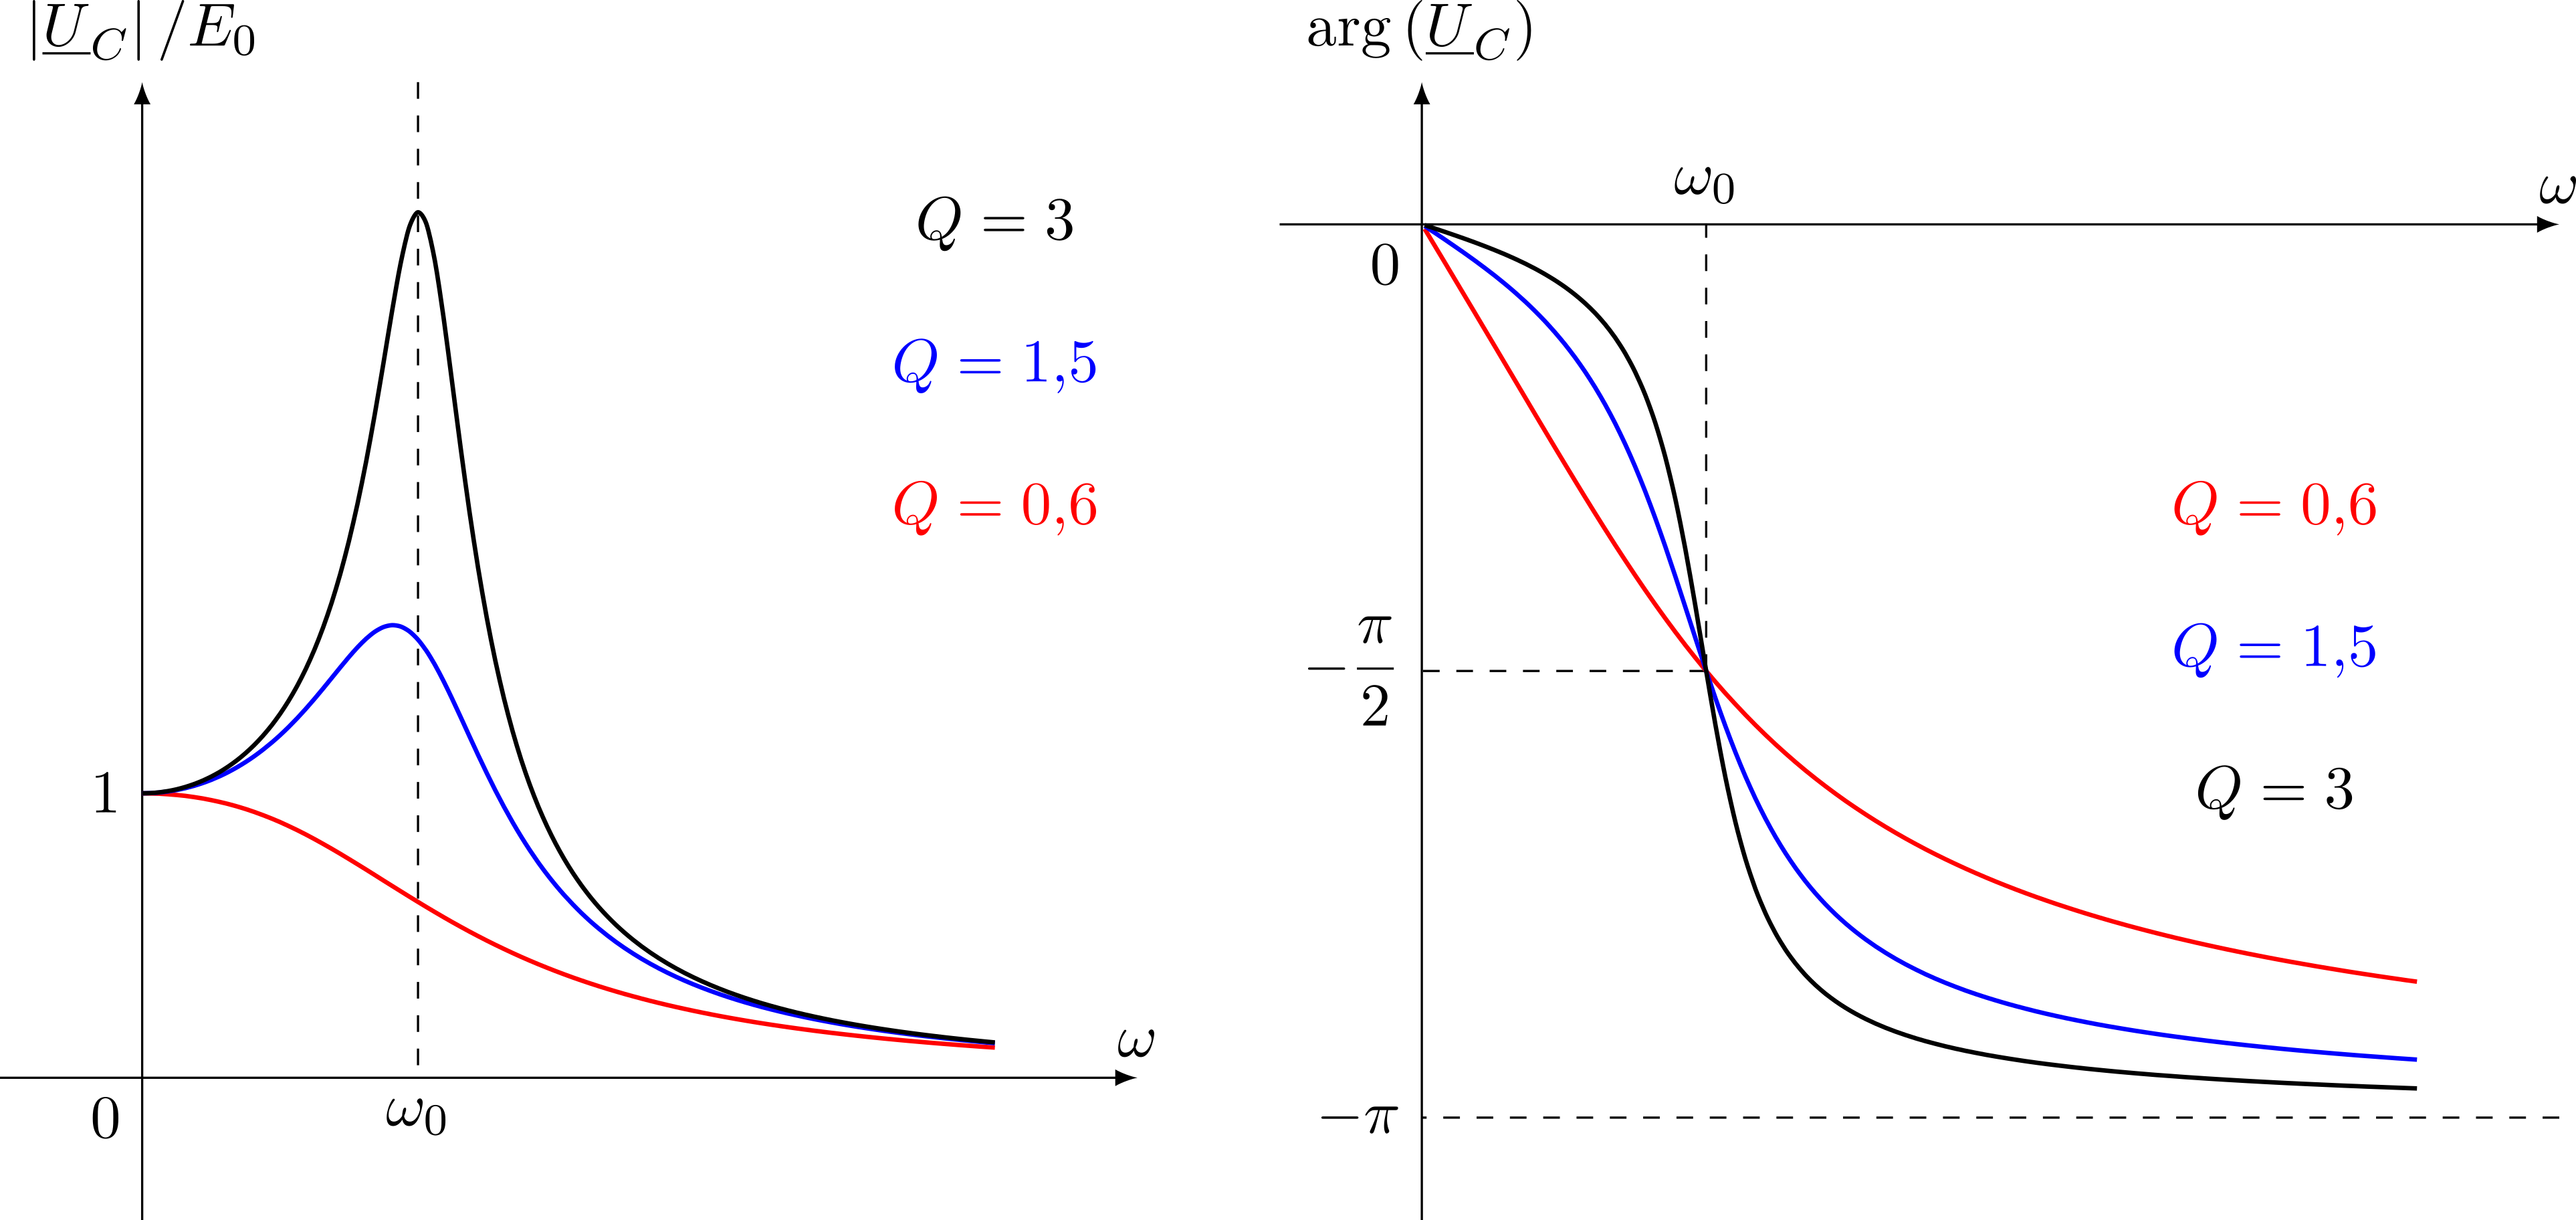
\includegraphics[width=0.9\linewidth]{rlc_u-ampphase}
	}
	\captionof{figure}{Amplitude et phase en fonction de $Q$ pour $\Uu_C$ en RLC
		série.}
\end{minipage}

\section{Exemple d'un oscillateur mécanique en RSF}
\subsection{Présentation}
\begin{tcb}(defi)<lft>{Situation initiale}
	\begin{description}
		\item[Système] : point matériel $M$ de masse $m$ relié à un ressort
		      horizontal \textbf{idéal}.
		\item[Référentiel] : $\Rc_{\rm sol} (O,x,y,t)$~;
	\end{description}
	\centers{\fbox{Soit $x = \ell - \ell_0$ la position de la masse}}
	\bigbreak
	\begin{minipage}{0.55\linewidth}
		\textbf{Bilan des forces}~:
		\begin{enumerate}
			\item
			      \psw{
				      Poids $\Pf = -mg\uy$~;
			      }
			\item
			      \psw{
				      Réaction du support $\vv{R} = R\uy$~;
			      }
			\item
			      \psw{
				      Force de rappel du ressort $\vv*{F}{\rm ressort} = -kx\ux$~;
			      }
			\item
			      \psw{
				      Force de frottement fluide $\vv*{F}{\rm frott} = -\alpha\vf$~;
			      }
			\item
			      \psw{
				      \textbf{Force excitatrice} $\ff_e = F_0\cos(\wt)\ux$.
			      }
		\end{enumerate}
	\end{minipage}
	\begin{minipage}{0.45\linewidth}
		\begin{center}
			\sswitch{
				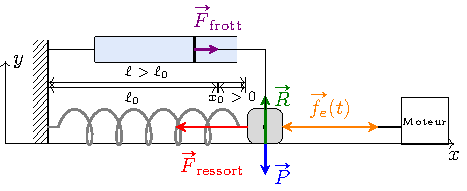
\includegraphics[width=\linewidth, draft=true]{ressort-horiz}
			}{
				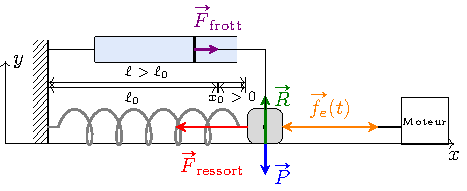
\includegraphics[width=\linewidth]{ressort-horiz}
			}
			\vspace{-15pt}
			\captionof{figure}{Schéma du ressort en RSF.}
		\end{center}
	\end{minipage}

\end{tcb}

\subsection{Étude de l'élongation}
\subsubsection{Équation}

\begin{tcb}(exem)<lft>{Calculs}
	Avec le PFD~:
	\psw{
		\begin{gather*}
			m\af = \Pf + \vv{R} + \Ff_{\rm ressort} + \Ff_{\rm frott} +\ff_e\\
			\Lra m\left(
			\begin{array}{c}
					\dv[2]{x}{t} \\
					0
				\end{array}
			\right)
			=
			\left(
			\begin{array}{c}
					-kx -\alpha v + F_0\cos(\wt) \\
					-mg + R
				\end{array}
			\right)
		\end{gather*}
		La projection sur $\uy$ montre que la réaction du support compense le poids.
		Sur l'axe $\ux$ on trouve
		\begin{gather*}
			m \dv[2]{x}{t} + \alpha \dv{x}{t} + kx = F_0\cos(\wt)
			\Lra
			\boxed{\xpp + \frac{\w_0}{Q}\xp + \w_0{}^2x =
				\frac{F_0}{m}\cos(\wt)}\\
			\qavec
			\boxed{\w_0 = \sqrt{\frac{k}{m}}}
			\qet
			Q = \frac{\sqrt{km}}{\alpha}
		\end{gather*}
	}
	\vspace{-15pt}
\end{tcb}
\begin{tcb}(prop)<lft>{Résultat}
	En passant en complexes,
	\psw{
		\begin{align*}
			\xul{X} & = \frac{F_0/m}{\w_0{}^2 - \w^2 + \jj \frac{\w\w_0}{Q}}
			\Lra
			\Aboxed{
			\xul{X} & = \frac{F_0}{m\w_0{}^2}\frac{1}{1 -
					\left( \dfrac{\w}{\w_0} \right)^2 +
					\jj\dfrac{\w}{Q\w_0}}
			}
		\end{align*}
	}
	\vspace{-15pt}
\end{tcb}

\subsubsection{Amplitude réelle et condition de résonance}
\begin{tcb}(prop)<lft>{Résultat}
	On trouve
	\psw{
		\begin{gather*}
			\boxed{
				X(\w)
				= \abs{\xul{X}}
				= \frac{F_0}{m\w_0{}^2}\frac{1}{
					\sqrt{\left( 1 - \left(\dfrac{\w}{\w_0}\right)^2 \right)^2
						+ \left(\dfrac{\w}{Q\w_0}\right)^2}}
			}
		\end{gather*}
	}
	Elle est maximale quand le dénominateur est minimal. Après calcul, on retrouve
	les résultats de l'excitation en tension~:
\end{tcb}
\begin{tcb}(ror){Conclusion}
	On trouve alors~:
	\begin{itemize}[leftmargin=60pt]
		\item[$\mathbf{Q \leq 1/\sqrt{2}}$] :
		      \psw{
			      \textbf{pas de résonance}, l'amplitude est maximale pour
			      \[\boxed{\w = 0 \qet X(0) = \frac{F_0}{m\w_0{}^2}}\]
		      }
		      \vspace{-15pt}
		\item[$\mathbf{Q > 1/\sqrt{2}}$] :
		      \psw{
			      il y a résonance, et l'amplitude est maximale pour
			      \[
				      \boxed{\w_r = \frac{\w_0}{Q} \sqrt{Q^{2} - \frac{1}{2}} < \w_0}
				      \qet
				      \boxed{X(\w_r) = \frac{F_0}{m\w_0{}^2}
					      \frac{Q}{\sqrt{1 - \frac{1}{4Q^2}}}}
			      \]
		      }
		      \vspace{-15pt}
		\item[$\mathbf{Q > 5}$] :
		      \psw{
			      \[
				      \boxed{\w_r \approx \w_0}
				      \qet
				      \boxed{X(\w_r) \approx \frac{QF_0}{k}}
			      \]
		      }
	\end{itemize}
	De ce résultat, nous observons qu'il \textbf{n'y a pas toujours résonance en
		élongation}, et que \textbf{la résonance est d'autant aiguë que $\mathbf{Q}$
		est élevé}.
\end{tcb}

Vous trouverez ici\footnote{\href{http://www.sciences.univ-nantes.fr/sites/genevieve\_tulloue/Meca/Oscillateurs/ressort\_rsf.php?typanim=Javascript}{http://www.sciences.univ-nantes.fr/sites/genevieve\_tulloue/Meca/Oscillateurs/ressort\_rsf.php?typanim=Javascript}} une animation interactive d'un système similaire avec un
ressort vertical.

\subsection{Résonance en vitesse}
\subsubsection{Équation}

À partir de $v(t) = \dv{x}{t} \Lra \Vu = \jw\Xu$~:
\begin{tcb}(exem)<lft>{Calculs}
	\psw{
		\begin{gather*}
			\xul{V}
			= \jj\w\xul{X}
			= \frac{F}{m\w_0} \frac{\jj\w}{\w_0 \left( 1 -
				\left( \dfrac{\w}{\w_0} \right)^2 + \jj\dfrac{\w}{Q\w_0} \right)}
			= \frac{F}{m\w_0} \frac{\w}{-\jj \left( \w_0 - \dfrac{\w^2}{\w_0} +
				\jj \dfrac{\w}{Q} \right)}\\
			\Lra
			\xul{V}
			= \frac{F}{m\w_0} \underbrace{\cancel{\frac{\w}{\w}}}_{=1}
			\frac{1}{-\jj \dfrac{\w_0}{\w} +\jj \dfrac{\w}{\w_0} - \jj^2
				\dfrac{1}{Q}}
			= \frac{F}{m\dfrac{\w_0}{Q}} \frac{1}{1 + \jj Q \left(
				\dfrac{\w}{\w_0} - \dfrac{\w_0}{\w}\right)}
		\end{gather*}
	}
	\vspace{-15pt}
\end{tcb}
\begin{tcb}(prop)<lft>{Résultat}
	Ainsi,
	\psw{
		\begin{equation*}
			\boxed{
				\xul{V} = \frac{F_0}{\alpha} \frac{1}{1 + \jj Q \left(
					\dfrac{\w}{\w_0} - \dfrac{\w_0}{\w}\right)}}
			\quad\text{car}\quad
			m \frac{\w_0}{Q} = \alpha
		\end{equation*}
	}
	\vspace{-15pt}
\end{tcb}
\begin{tcb}(ror){Conclusion}
	On trouve alors
	\[
		\psw{
			\boxed{
				V_{\max} = V(\w_0) = \frac{F_0}{\alpha}
			}
		}
		\qet
		\psw{
			\boxed{
				V\xrightarrow[\w\to0^+]{} 0
			}
		}
		\qet
		\psw{
			\boxed{
				V\xrightarrow[\w\to+\infty]{} 0
			}
		}
	\]
	De ce résultat, nous observons qu'il \textbf{n'y a pas de condition pour avoir
		résonance en vitesse}, et que \textbf{la pulsation de résonance est la
		pulsation propre du système}.
\end{tcb}
%On retrouve également $Q = \w_0/\D\w$ avec $\f(\w_r) = 0$.

\vspace{-15pt}
\section{Synthèse}
\begin{tcb}[label=ror:oscrsf-synth,
		tabularx*={\renewcommand{\arraystretch}{1.8}}{M{3cm}|Y|Y}]
	(ror){Synthèse résonances}
	\textbf{Grandeur} &
	Intensité/vitesse &
	Tension/élongation
	\\\hline
	\textbf{Existence} &
	\psw{Toujours}
	&
	\psw{$Q > 1/\sqrt{2}$}
	\\\hline
	\textbf{Pulsation de résonance} &
	\psw{$\w_0$}
	&
	\psw{$\w_r \lesssim \w_0$}
	\\\hdashline
	\textbf{Largeur de résonance} &
	\psw{$\D\w = \dfrac{\w_0}{Q}$}
	&
	\psw{$\D\w \approx\dfrac{\w_0}{Q}$}
	\\\hline
	\textbf{Aspects à $\w_r$} &
	\psw{
		Maximum d'amplitude\smallbreak
		Déphasage nul, $\f = 0$
	}
	&
	\psw{
		Maximum d'amplitude
	}
	\\\hdashline
	\textbf{Aspects à $\w_0$} &
	\psw{
		Résonance
	}
	&
	\psw{
		Sortie = $Q\times$entrée\smallbreak
		Quadrature de phase, $\f = -\dfrac{\pi}{2}$
	}
	\\\hline
	\textbf{Courbes d'amplitude} &
	\sswitch{
		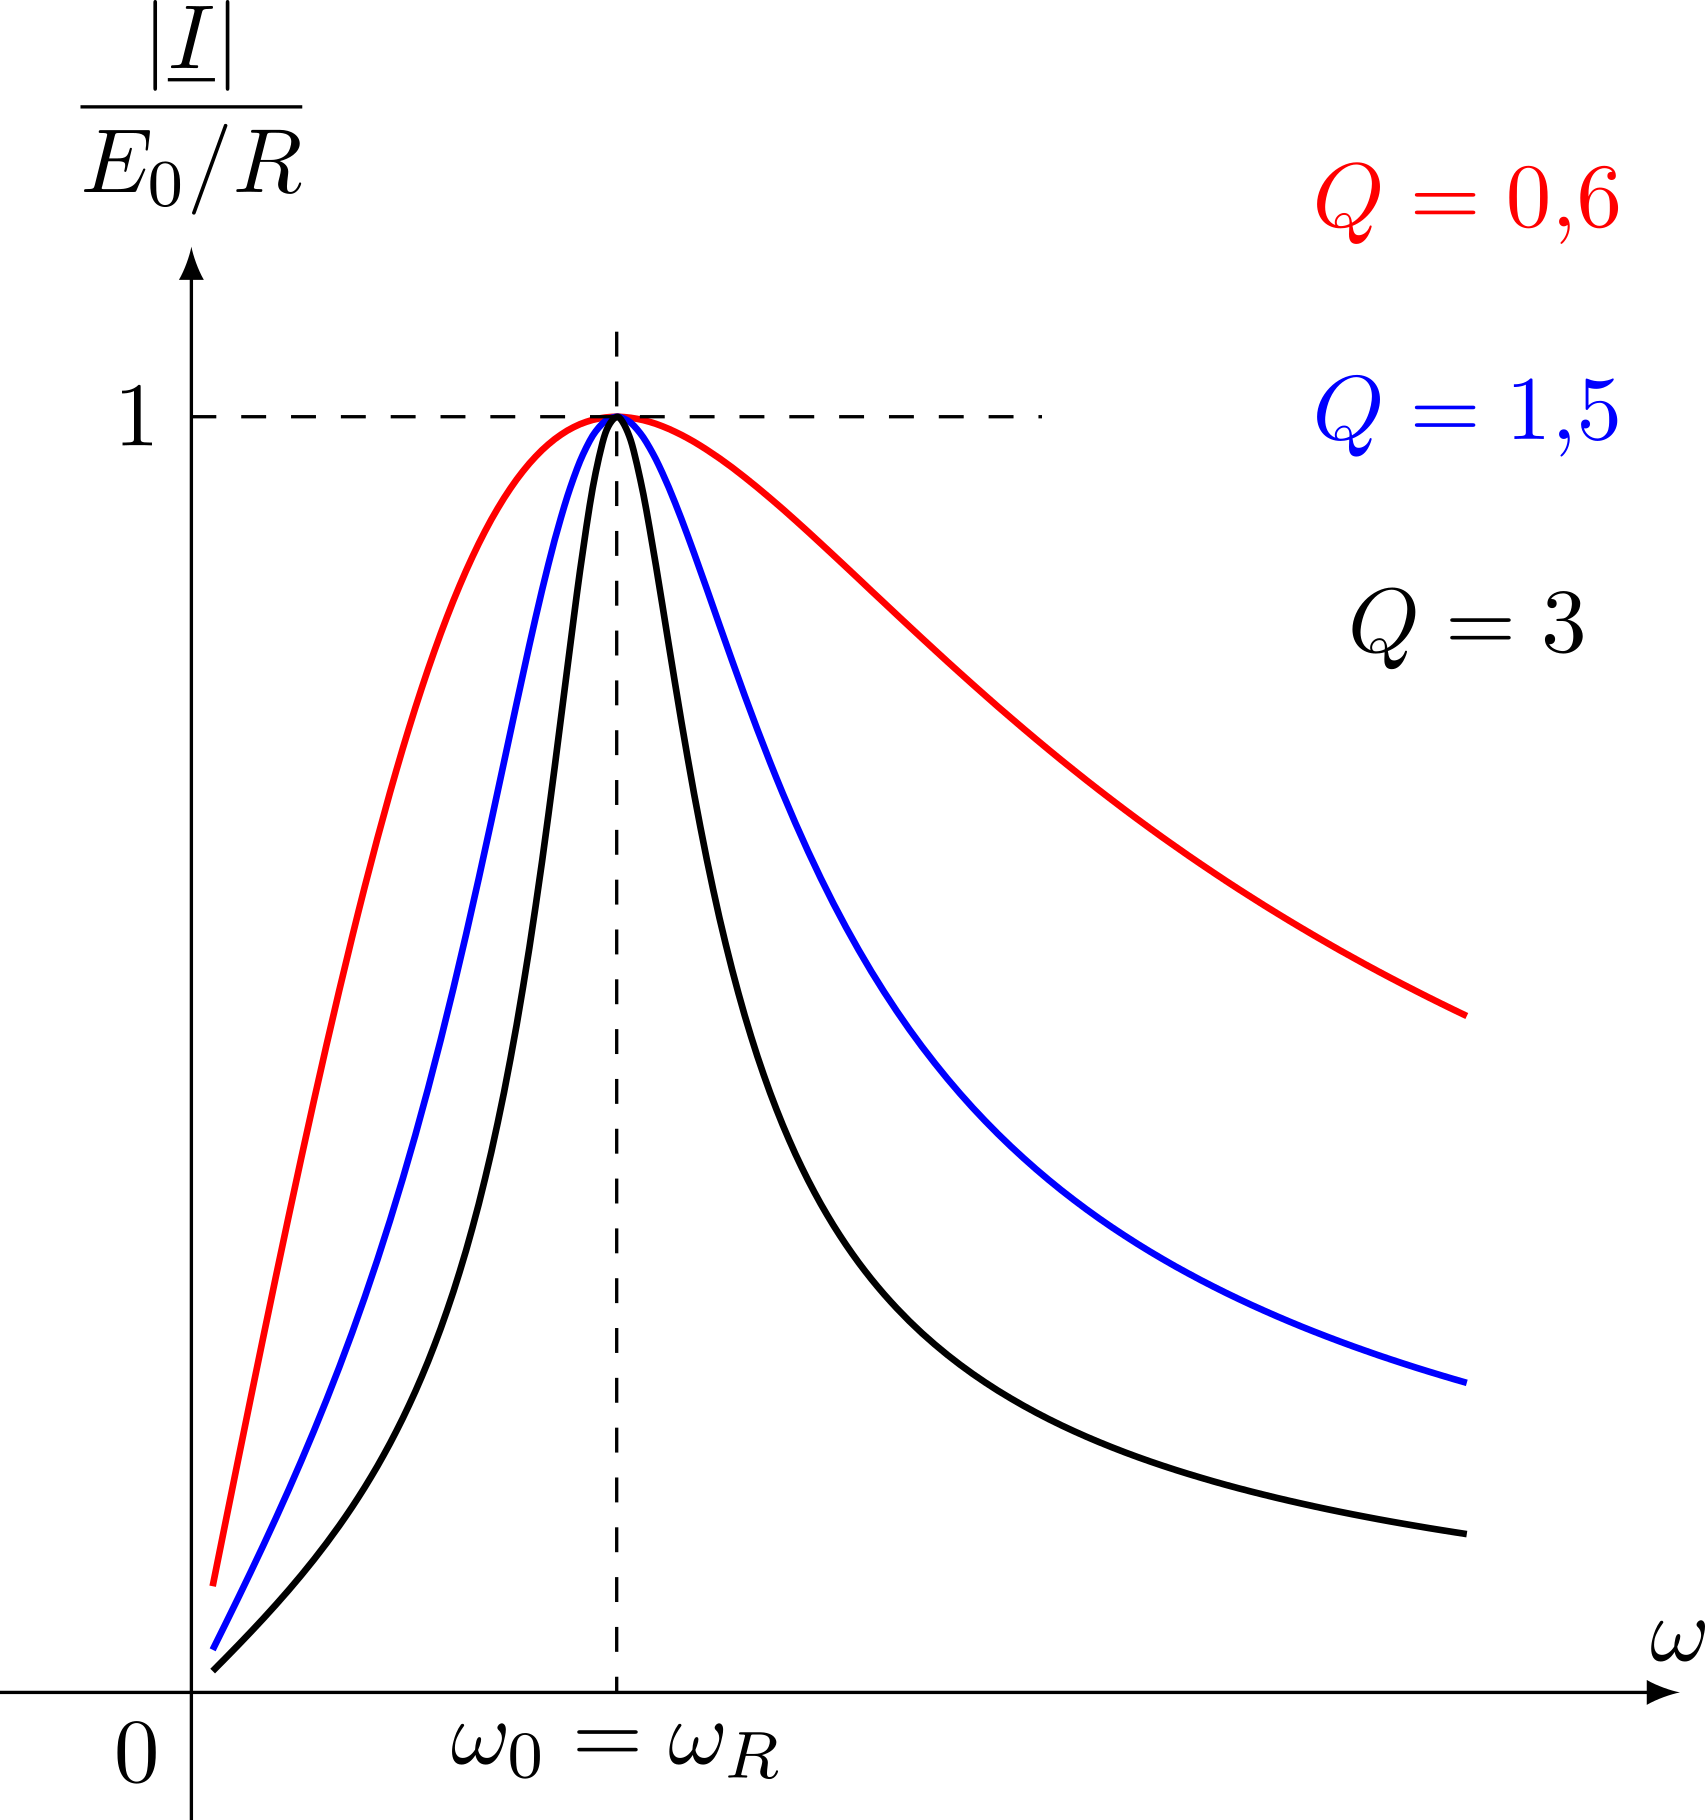
\includegraphics[width=.6\linewidth, draft=true]{rlc_i-amp}
	}{
		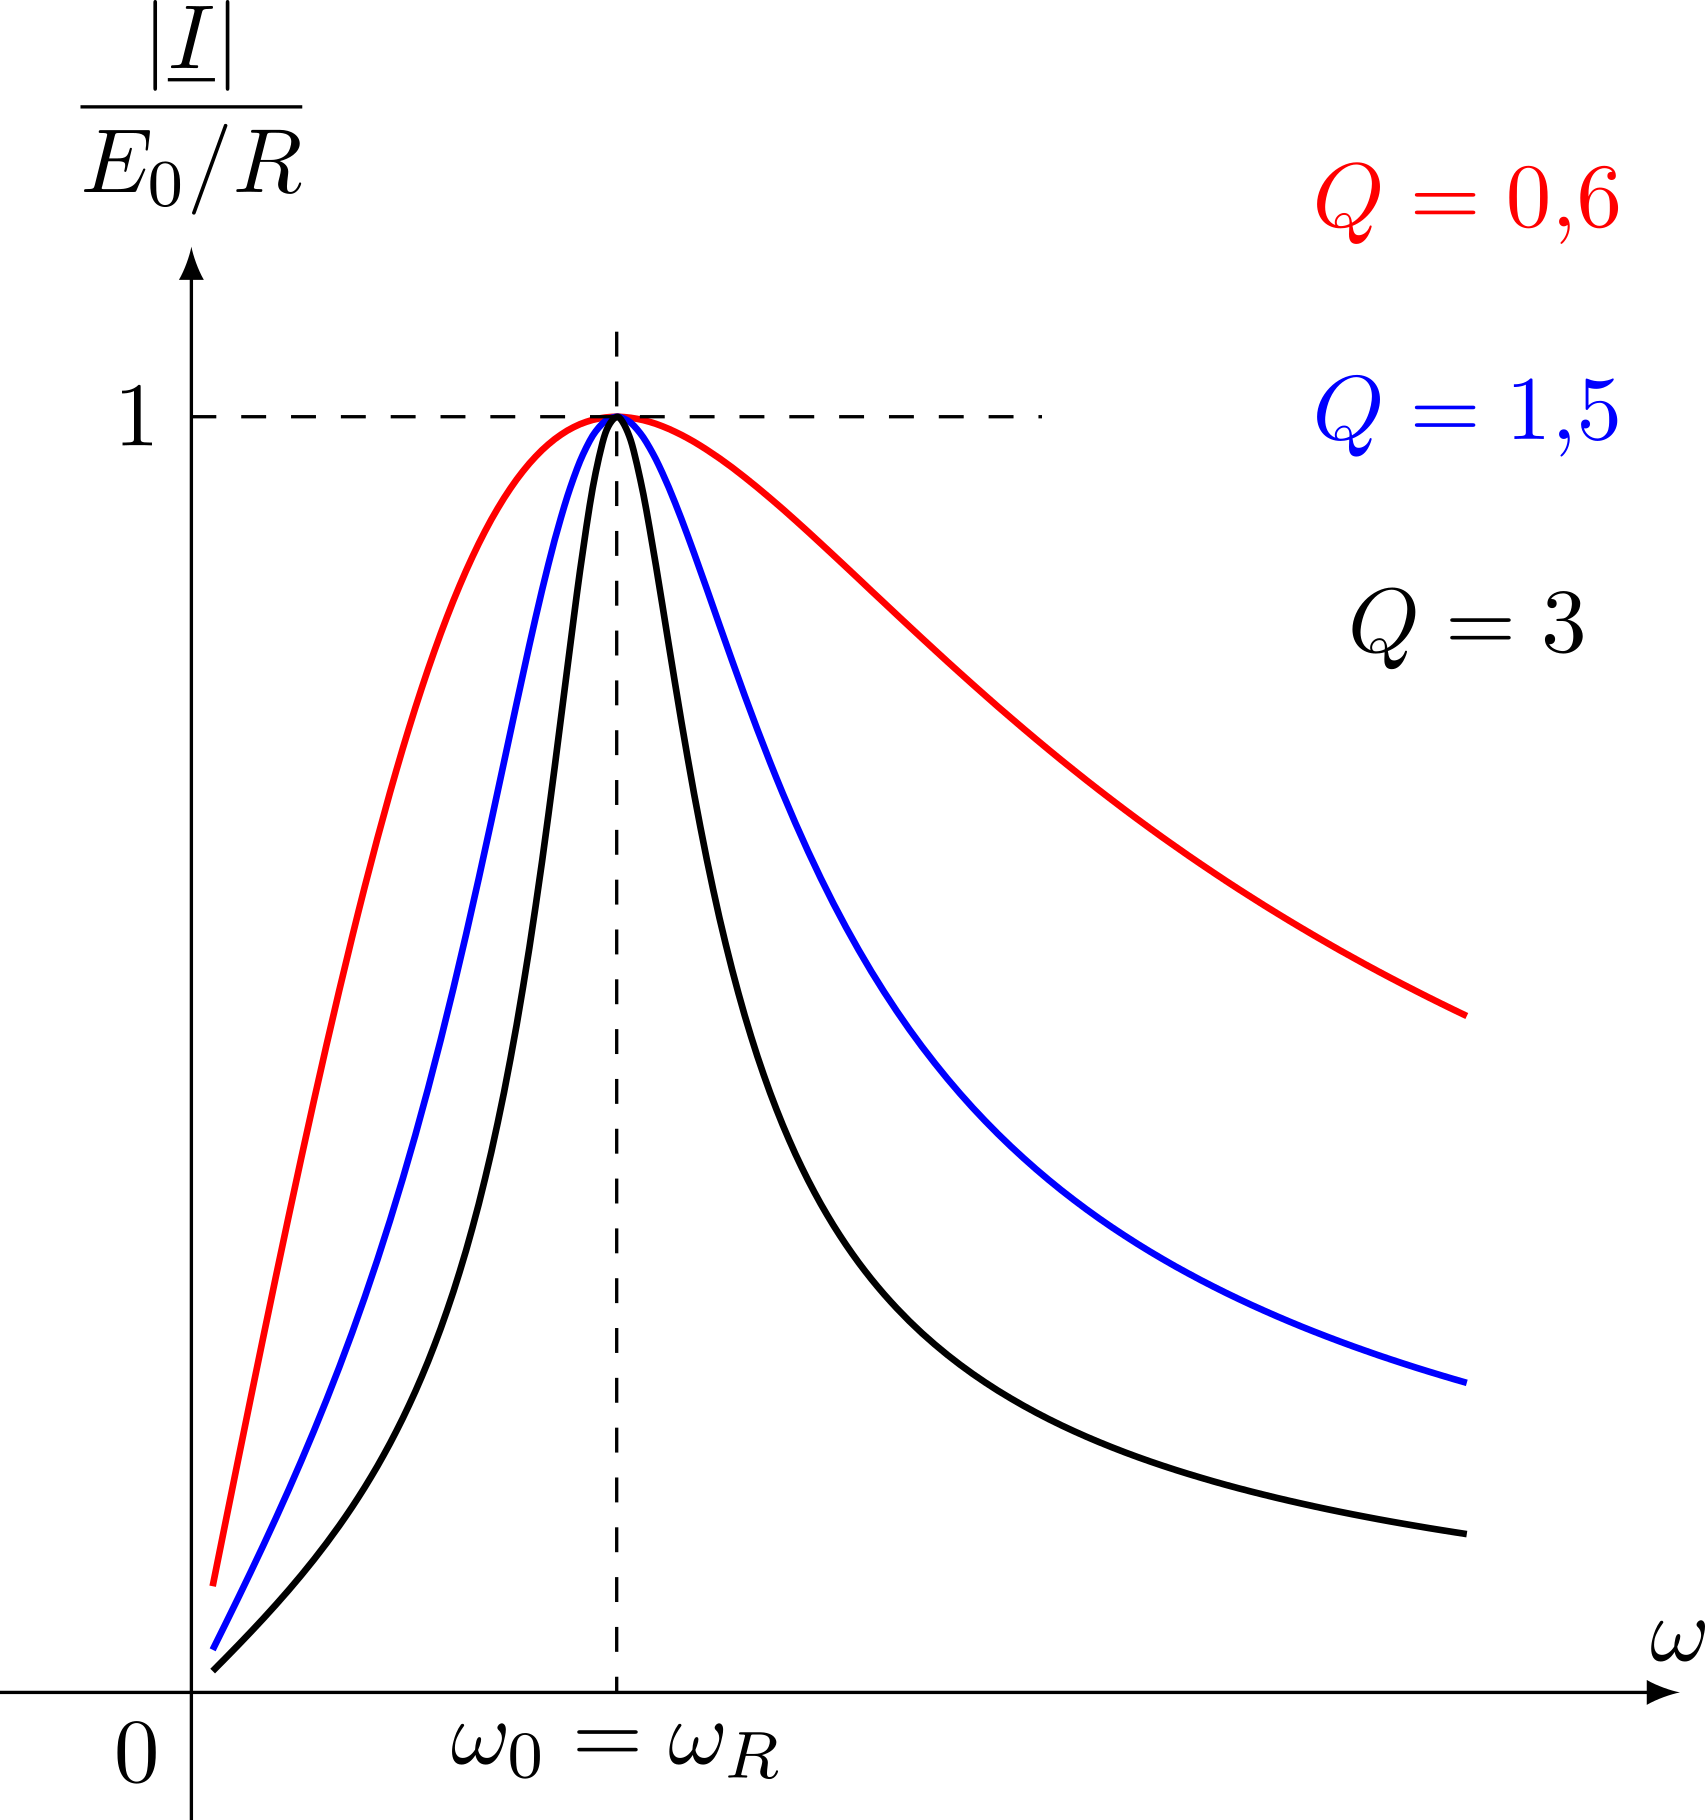
\includegraphics[width=.6\linewidth]{rlc_i-amp}
	}

	&
	\sswitch{
		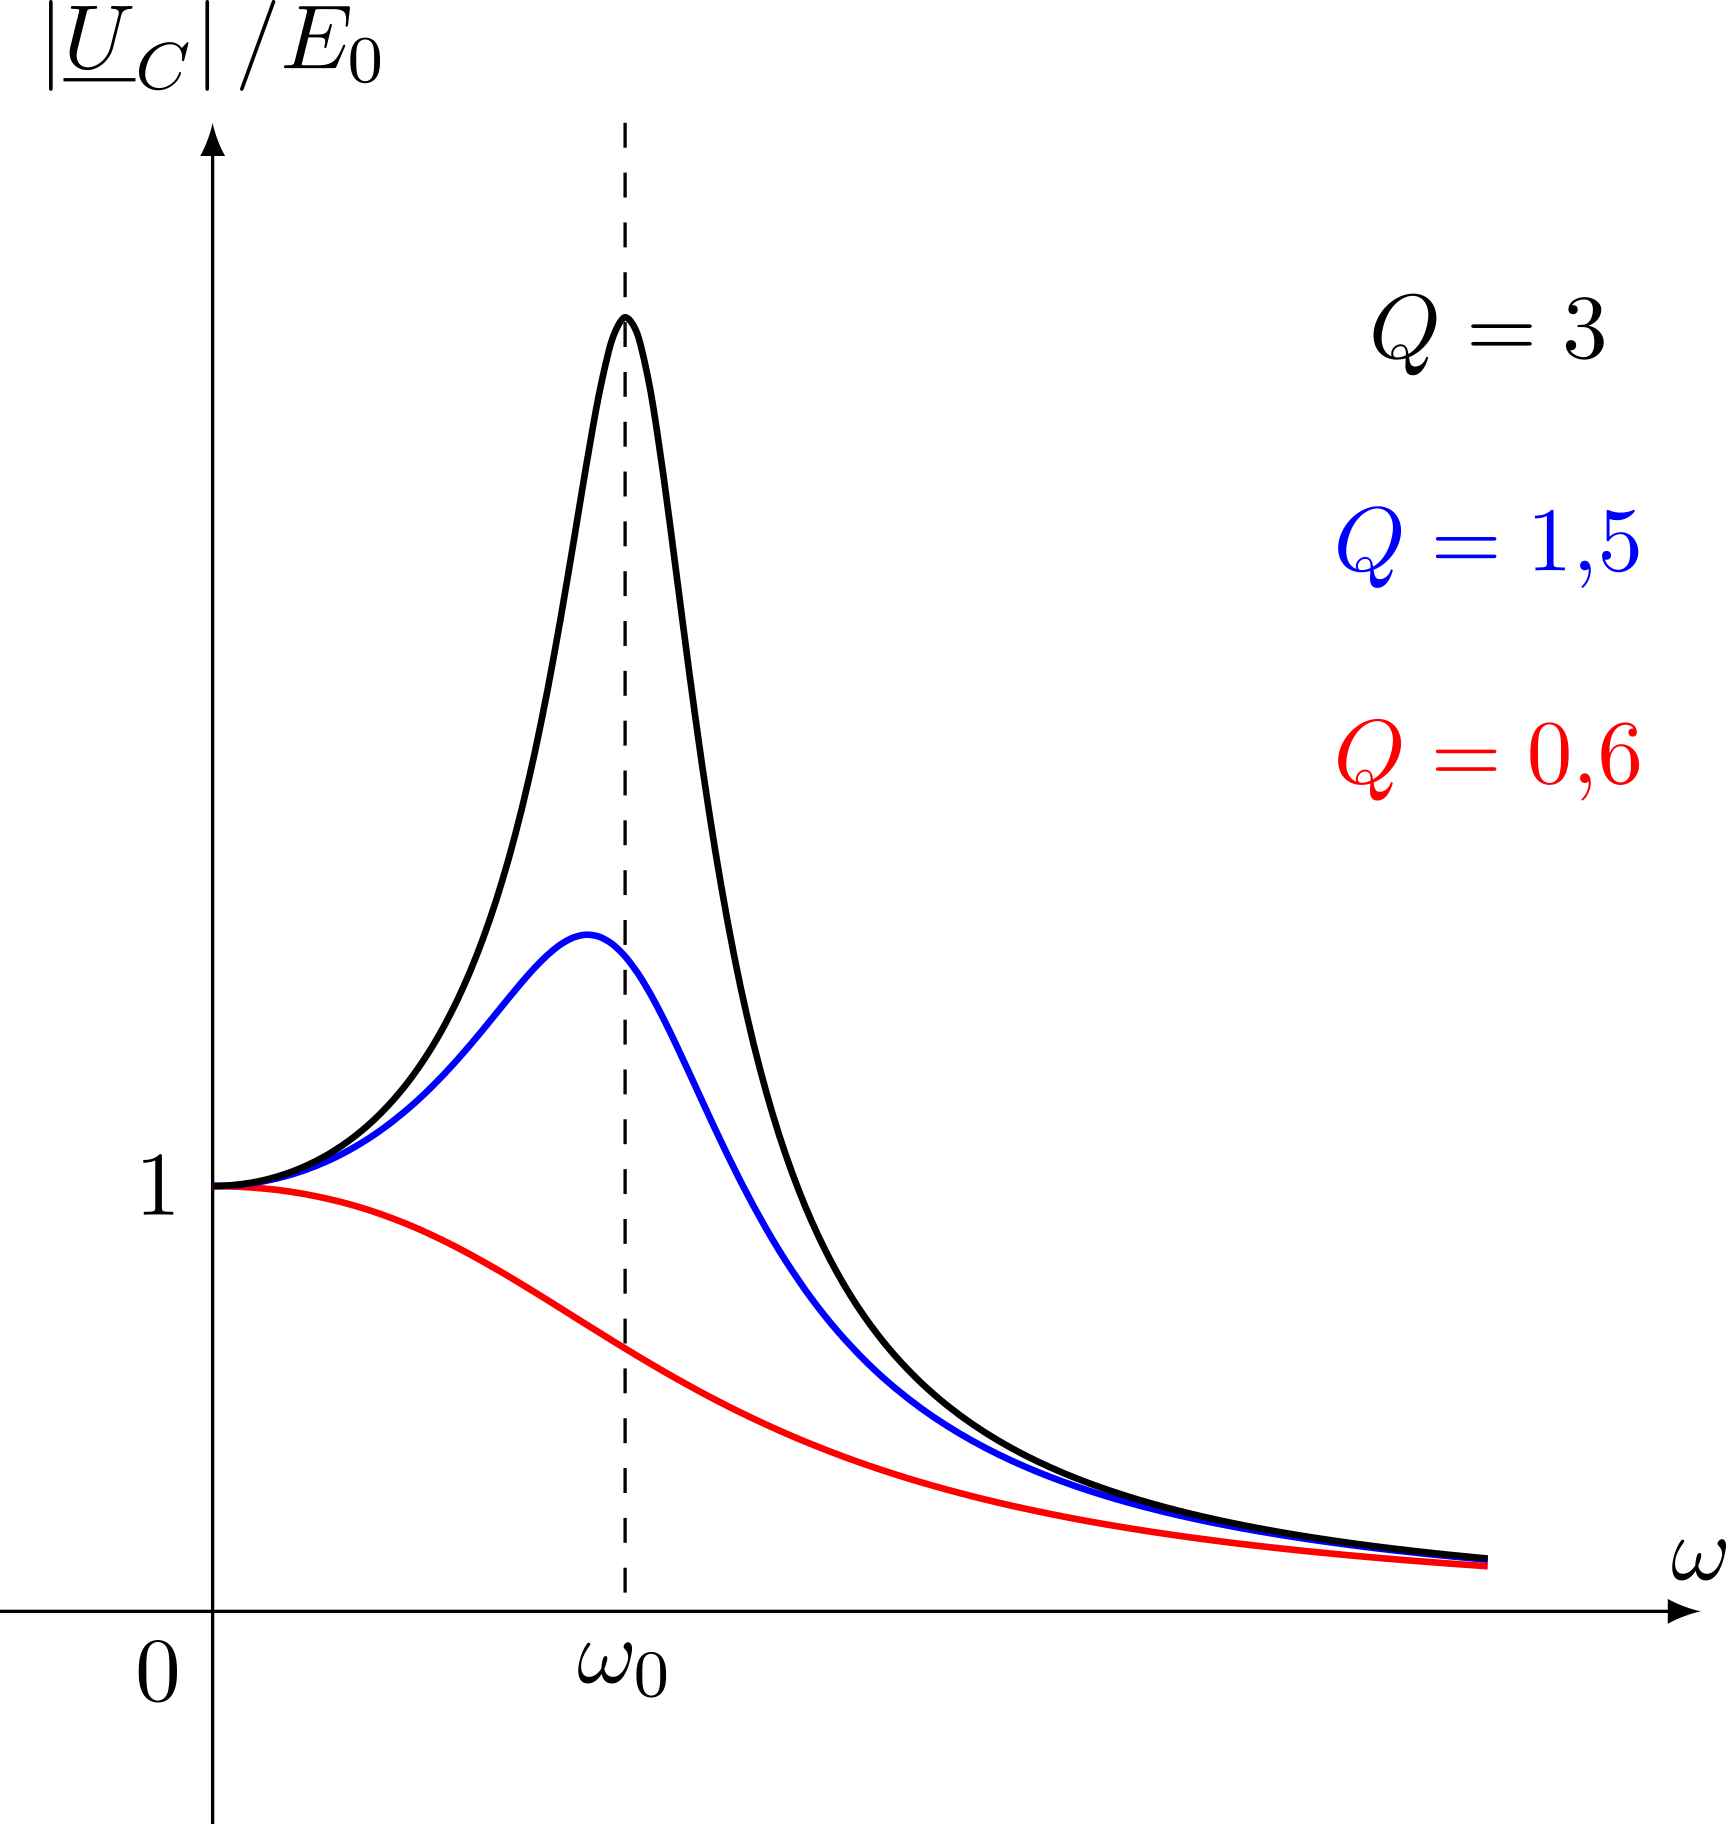
\includegraphics[width=.6\linewidth, draft=true]{rlc_u-amp}
	}{
		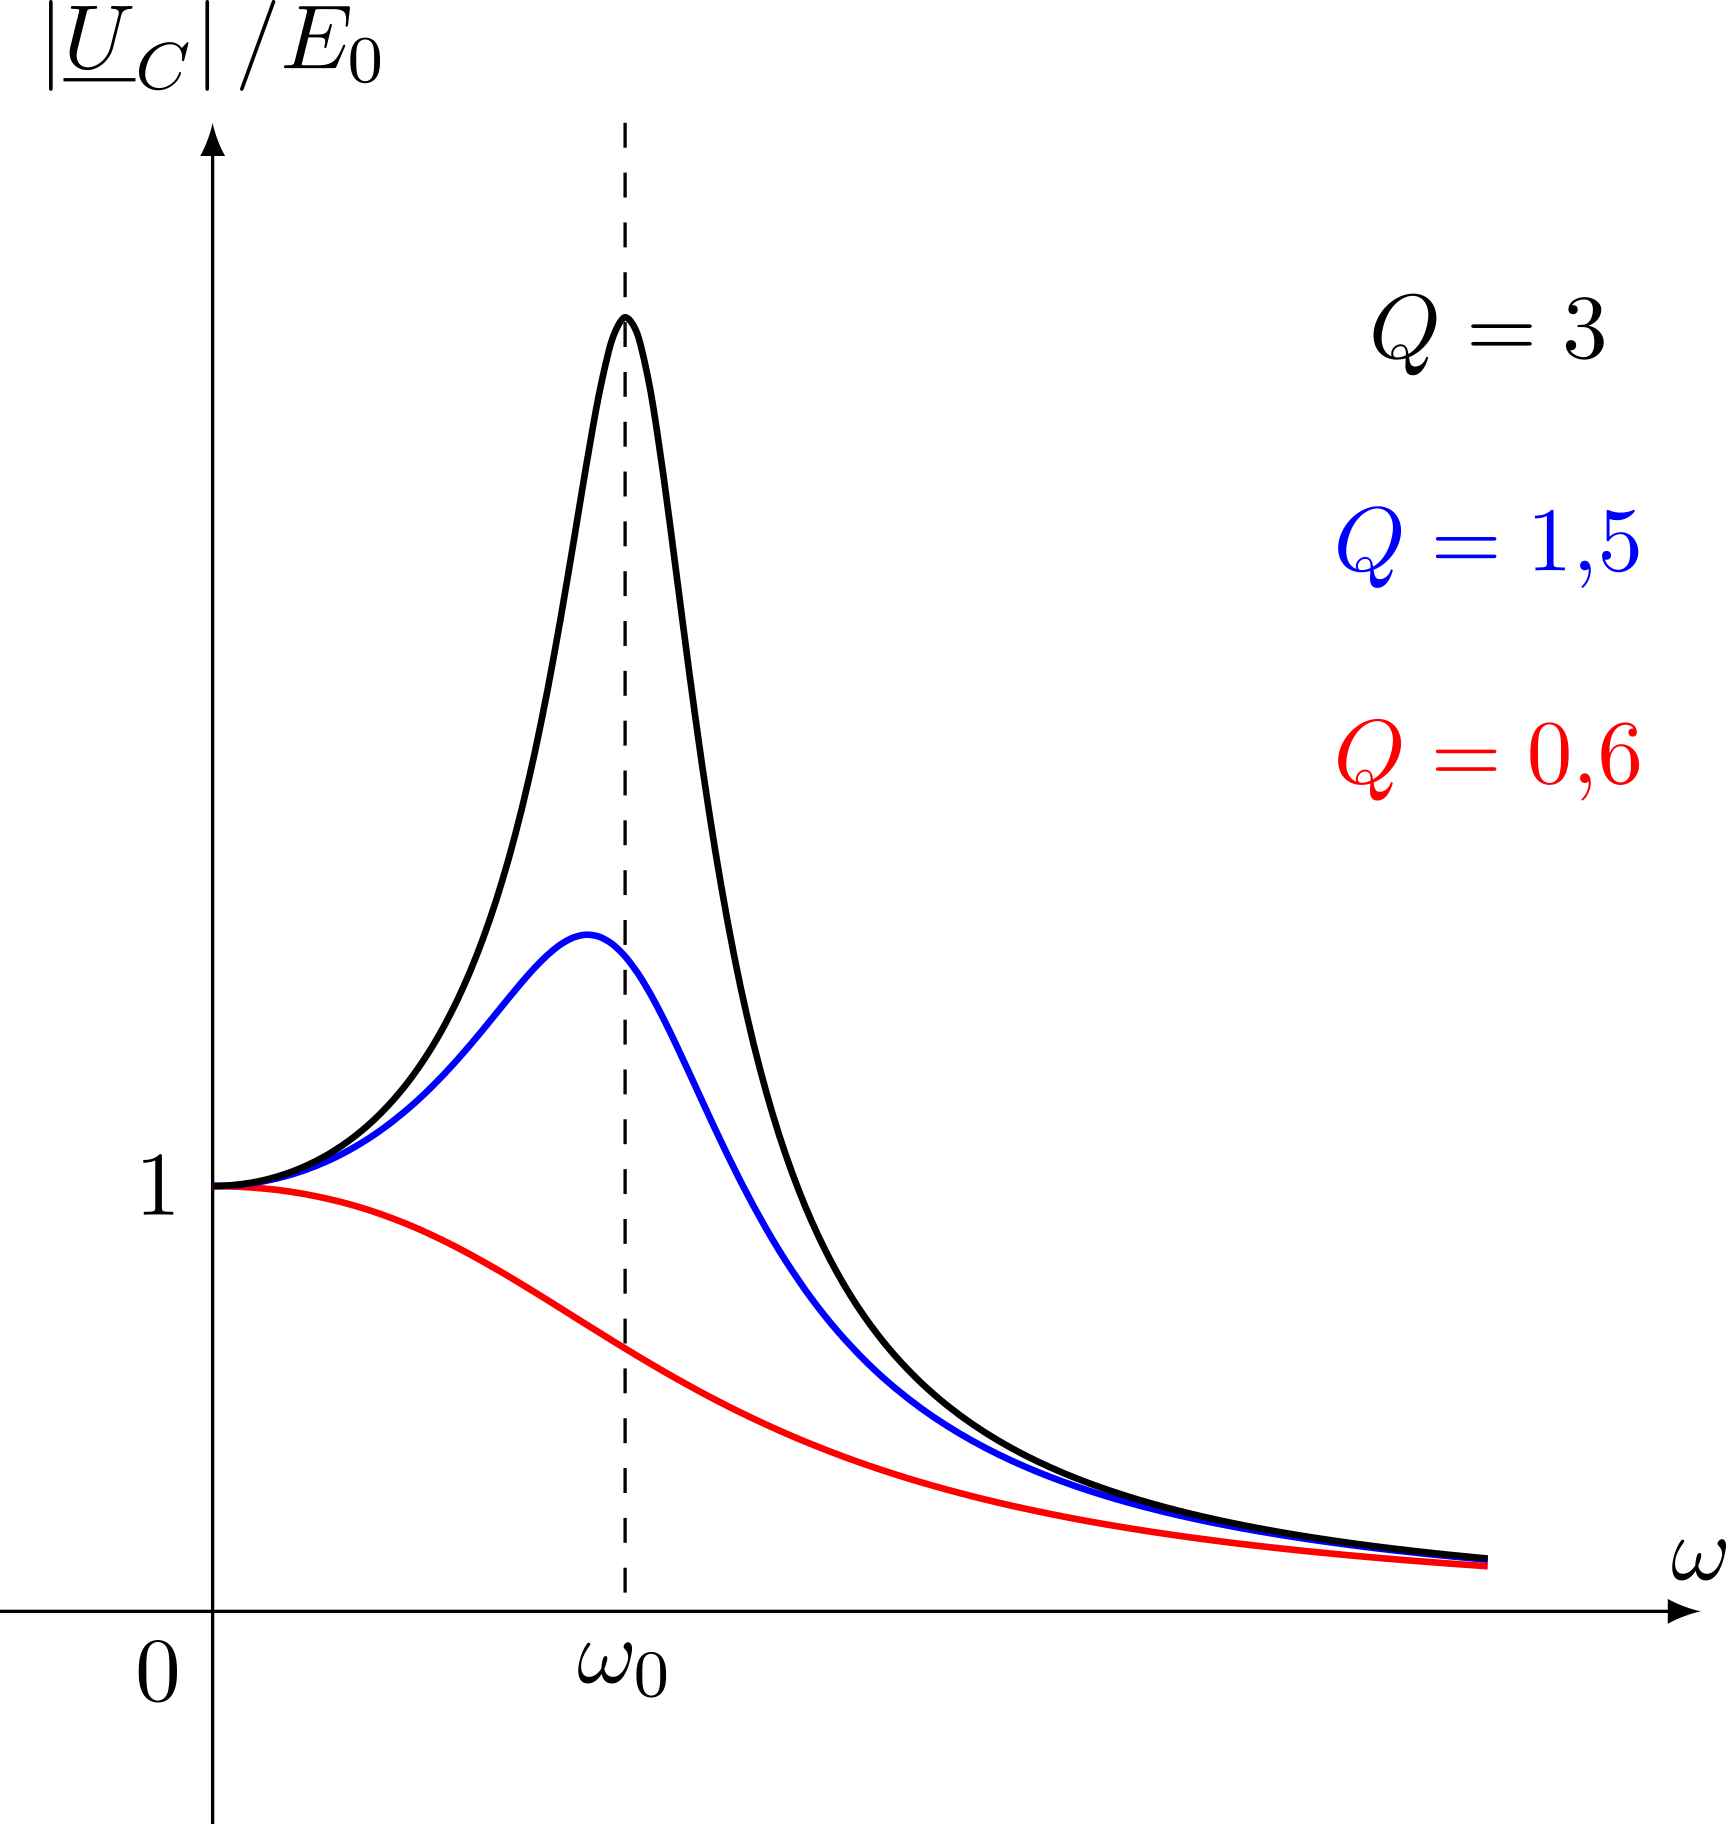
\includegraphics[width=.6\linewidth]{rlc_u-amp}
	}

	\\\hdashline
	\textbf{Courbes de phase} &
	\sswitch{
		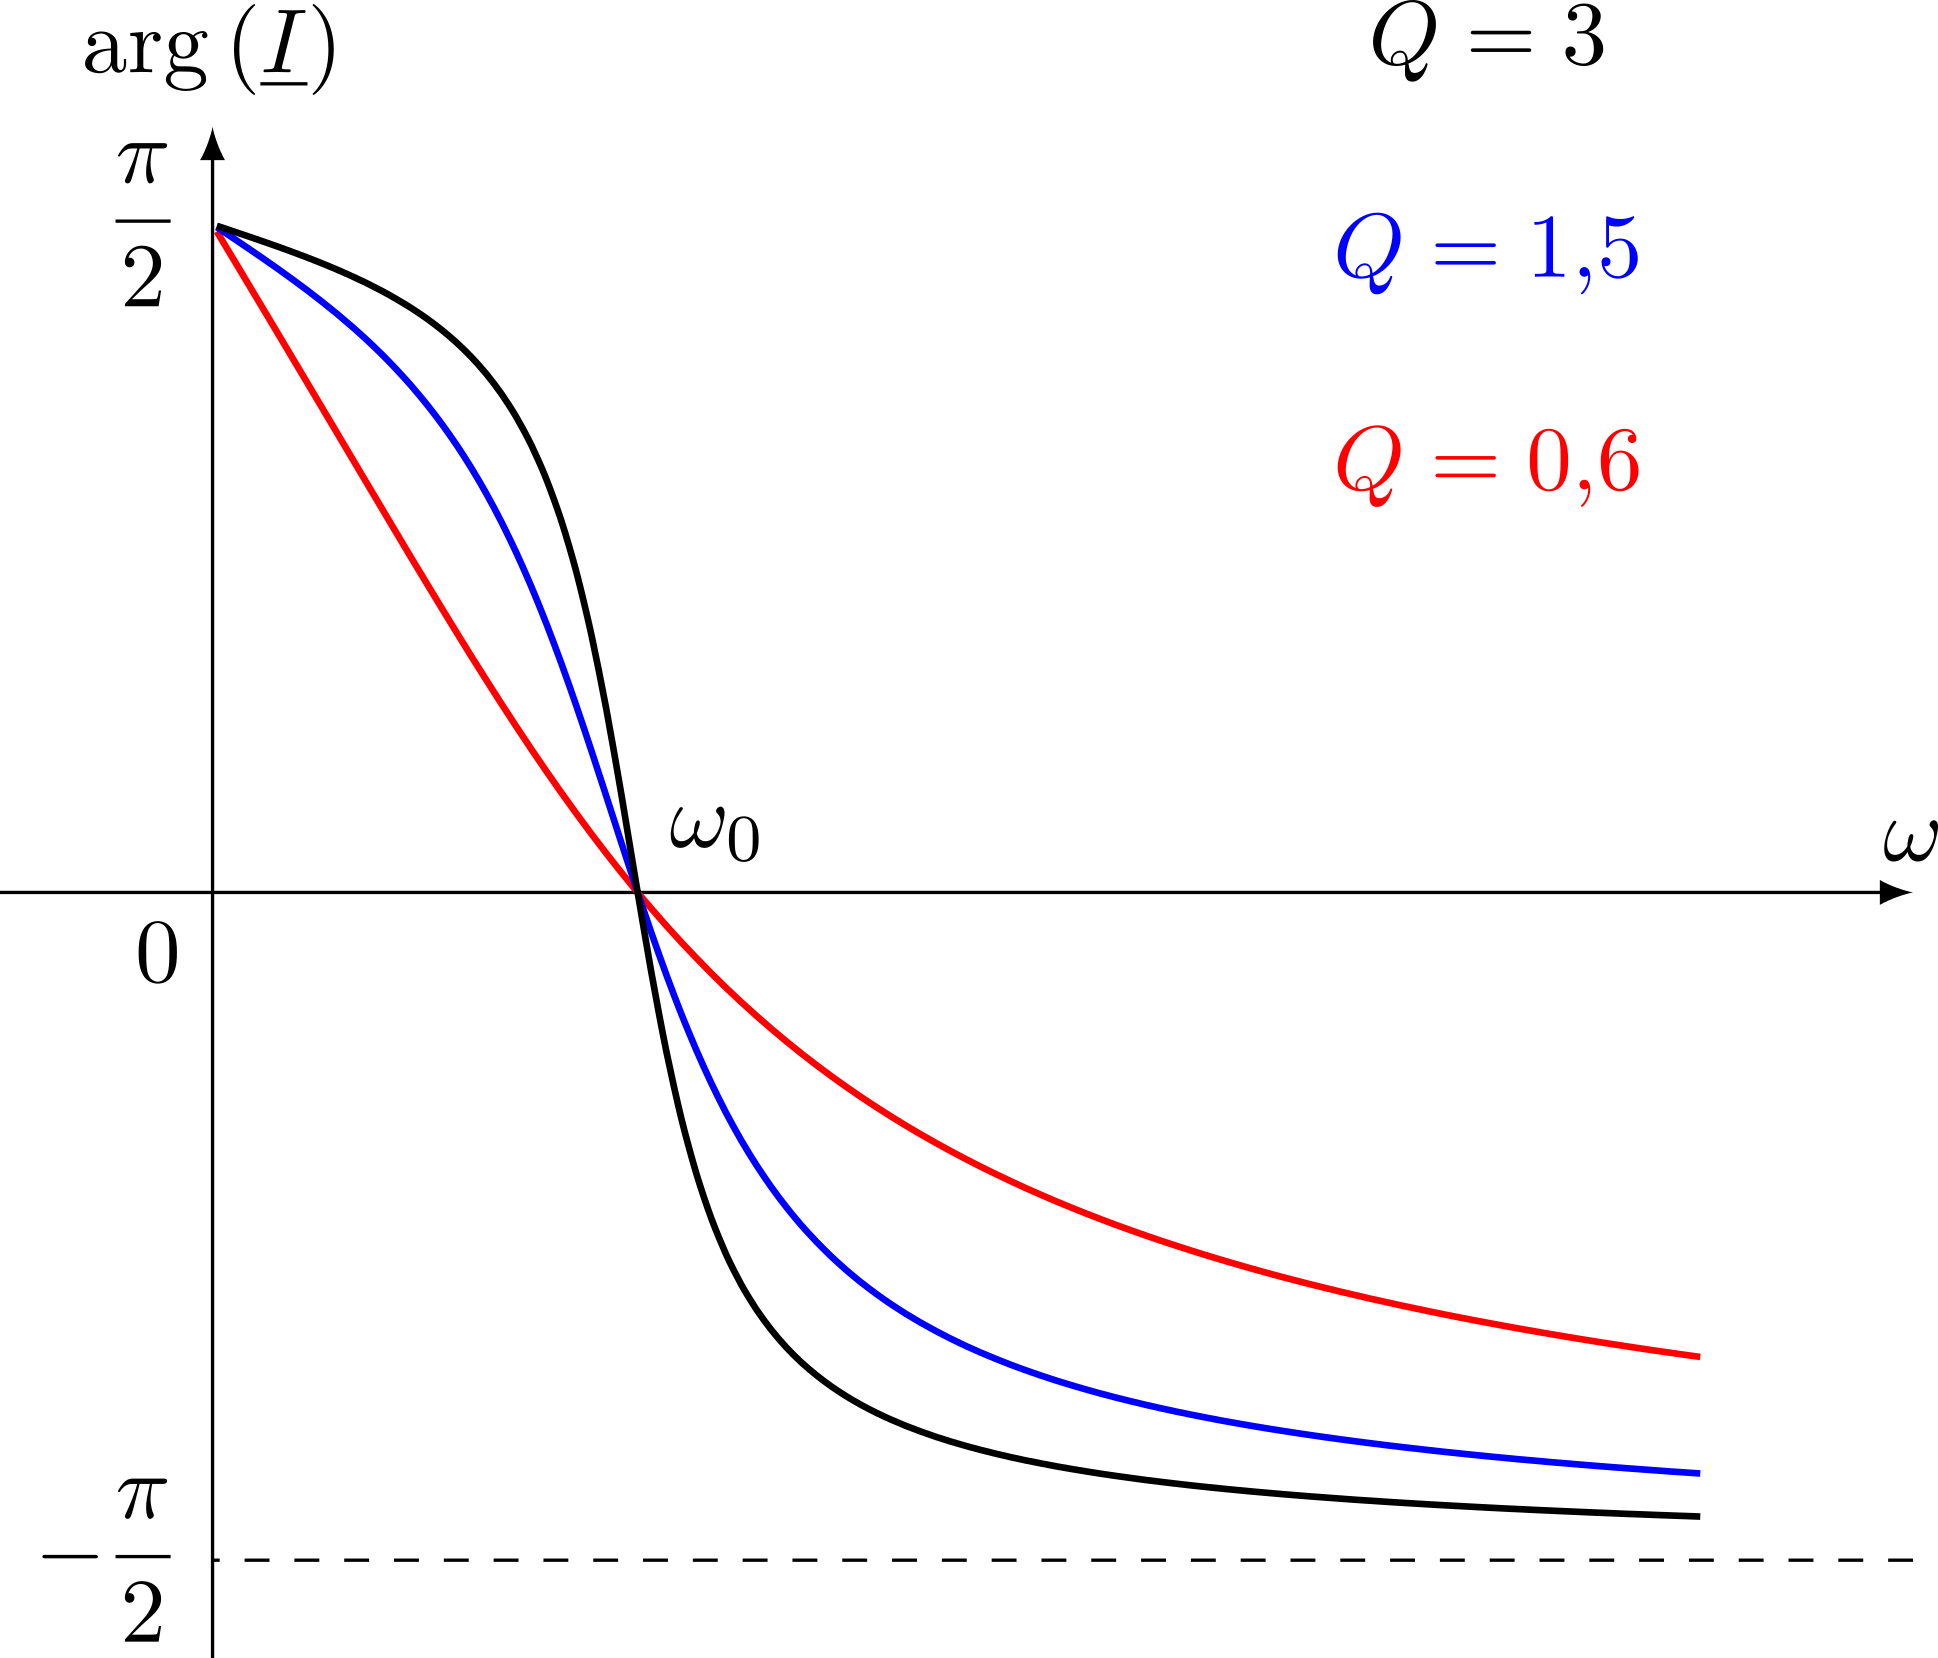
\includegraphics[width=.6\linewidth, draft=true]{rlc_i-phase}
	}{
		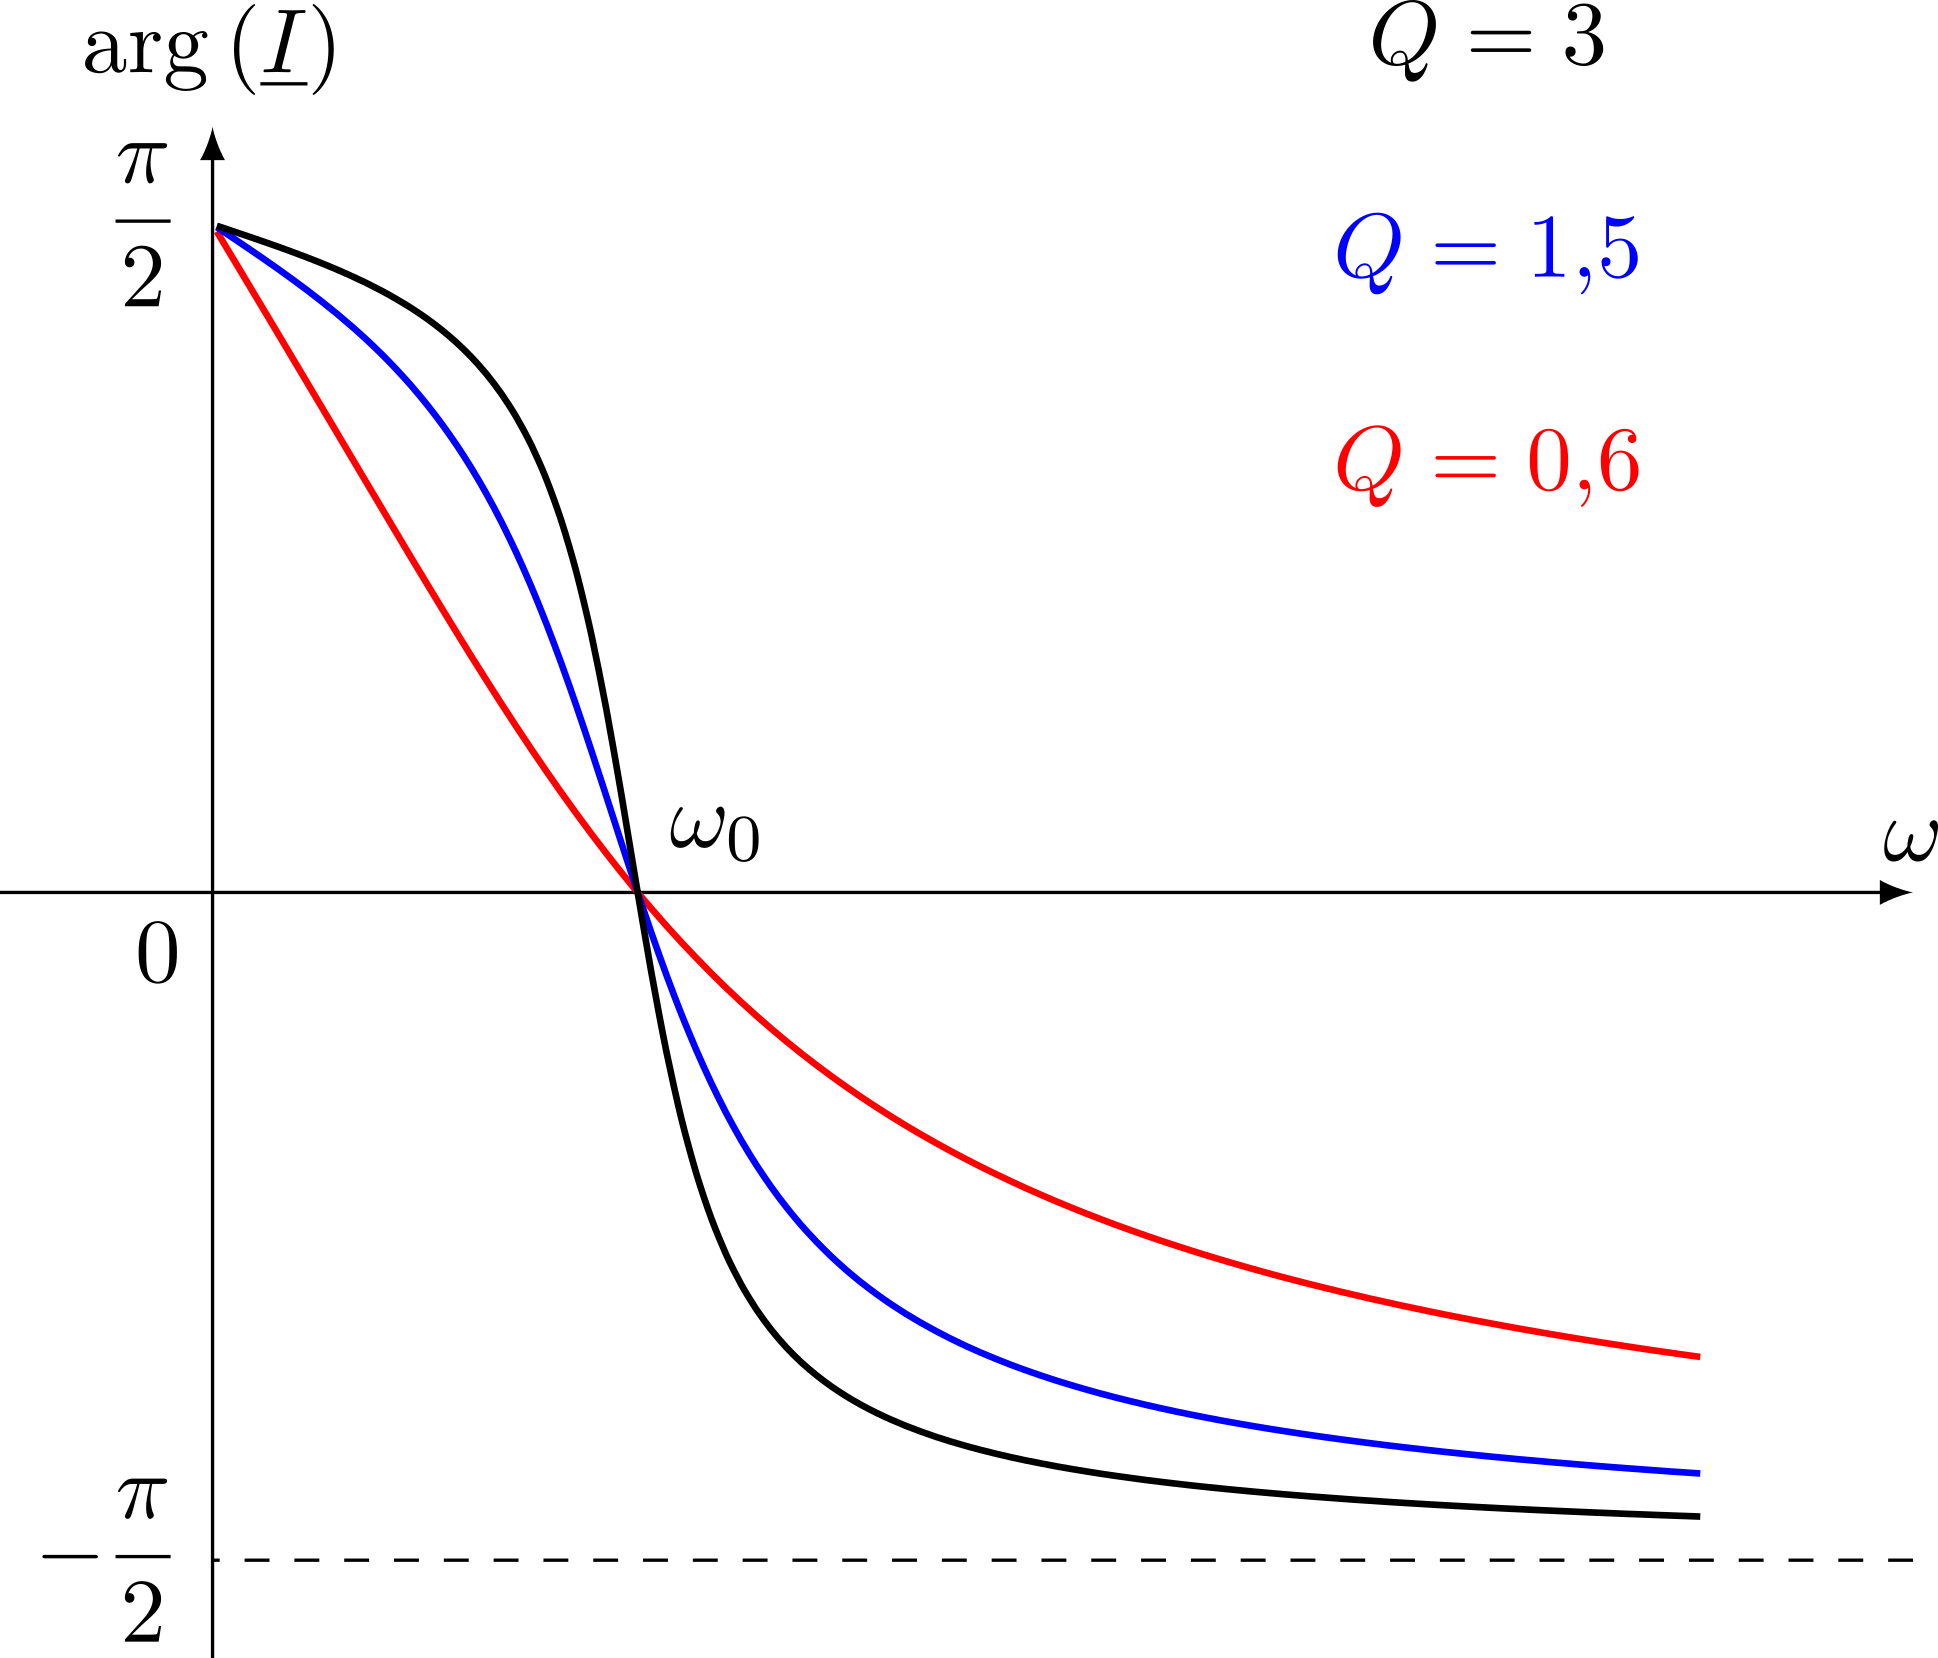
\includegraphics[width=.6\linewidth]{rlc_i-phase}
	}
	&
	\sswitch{
		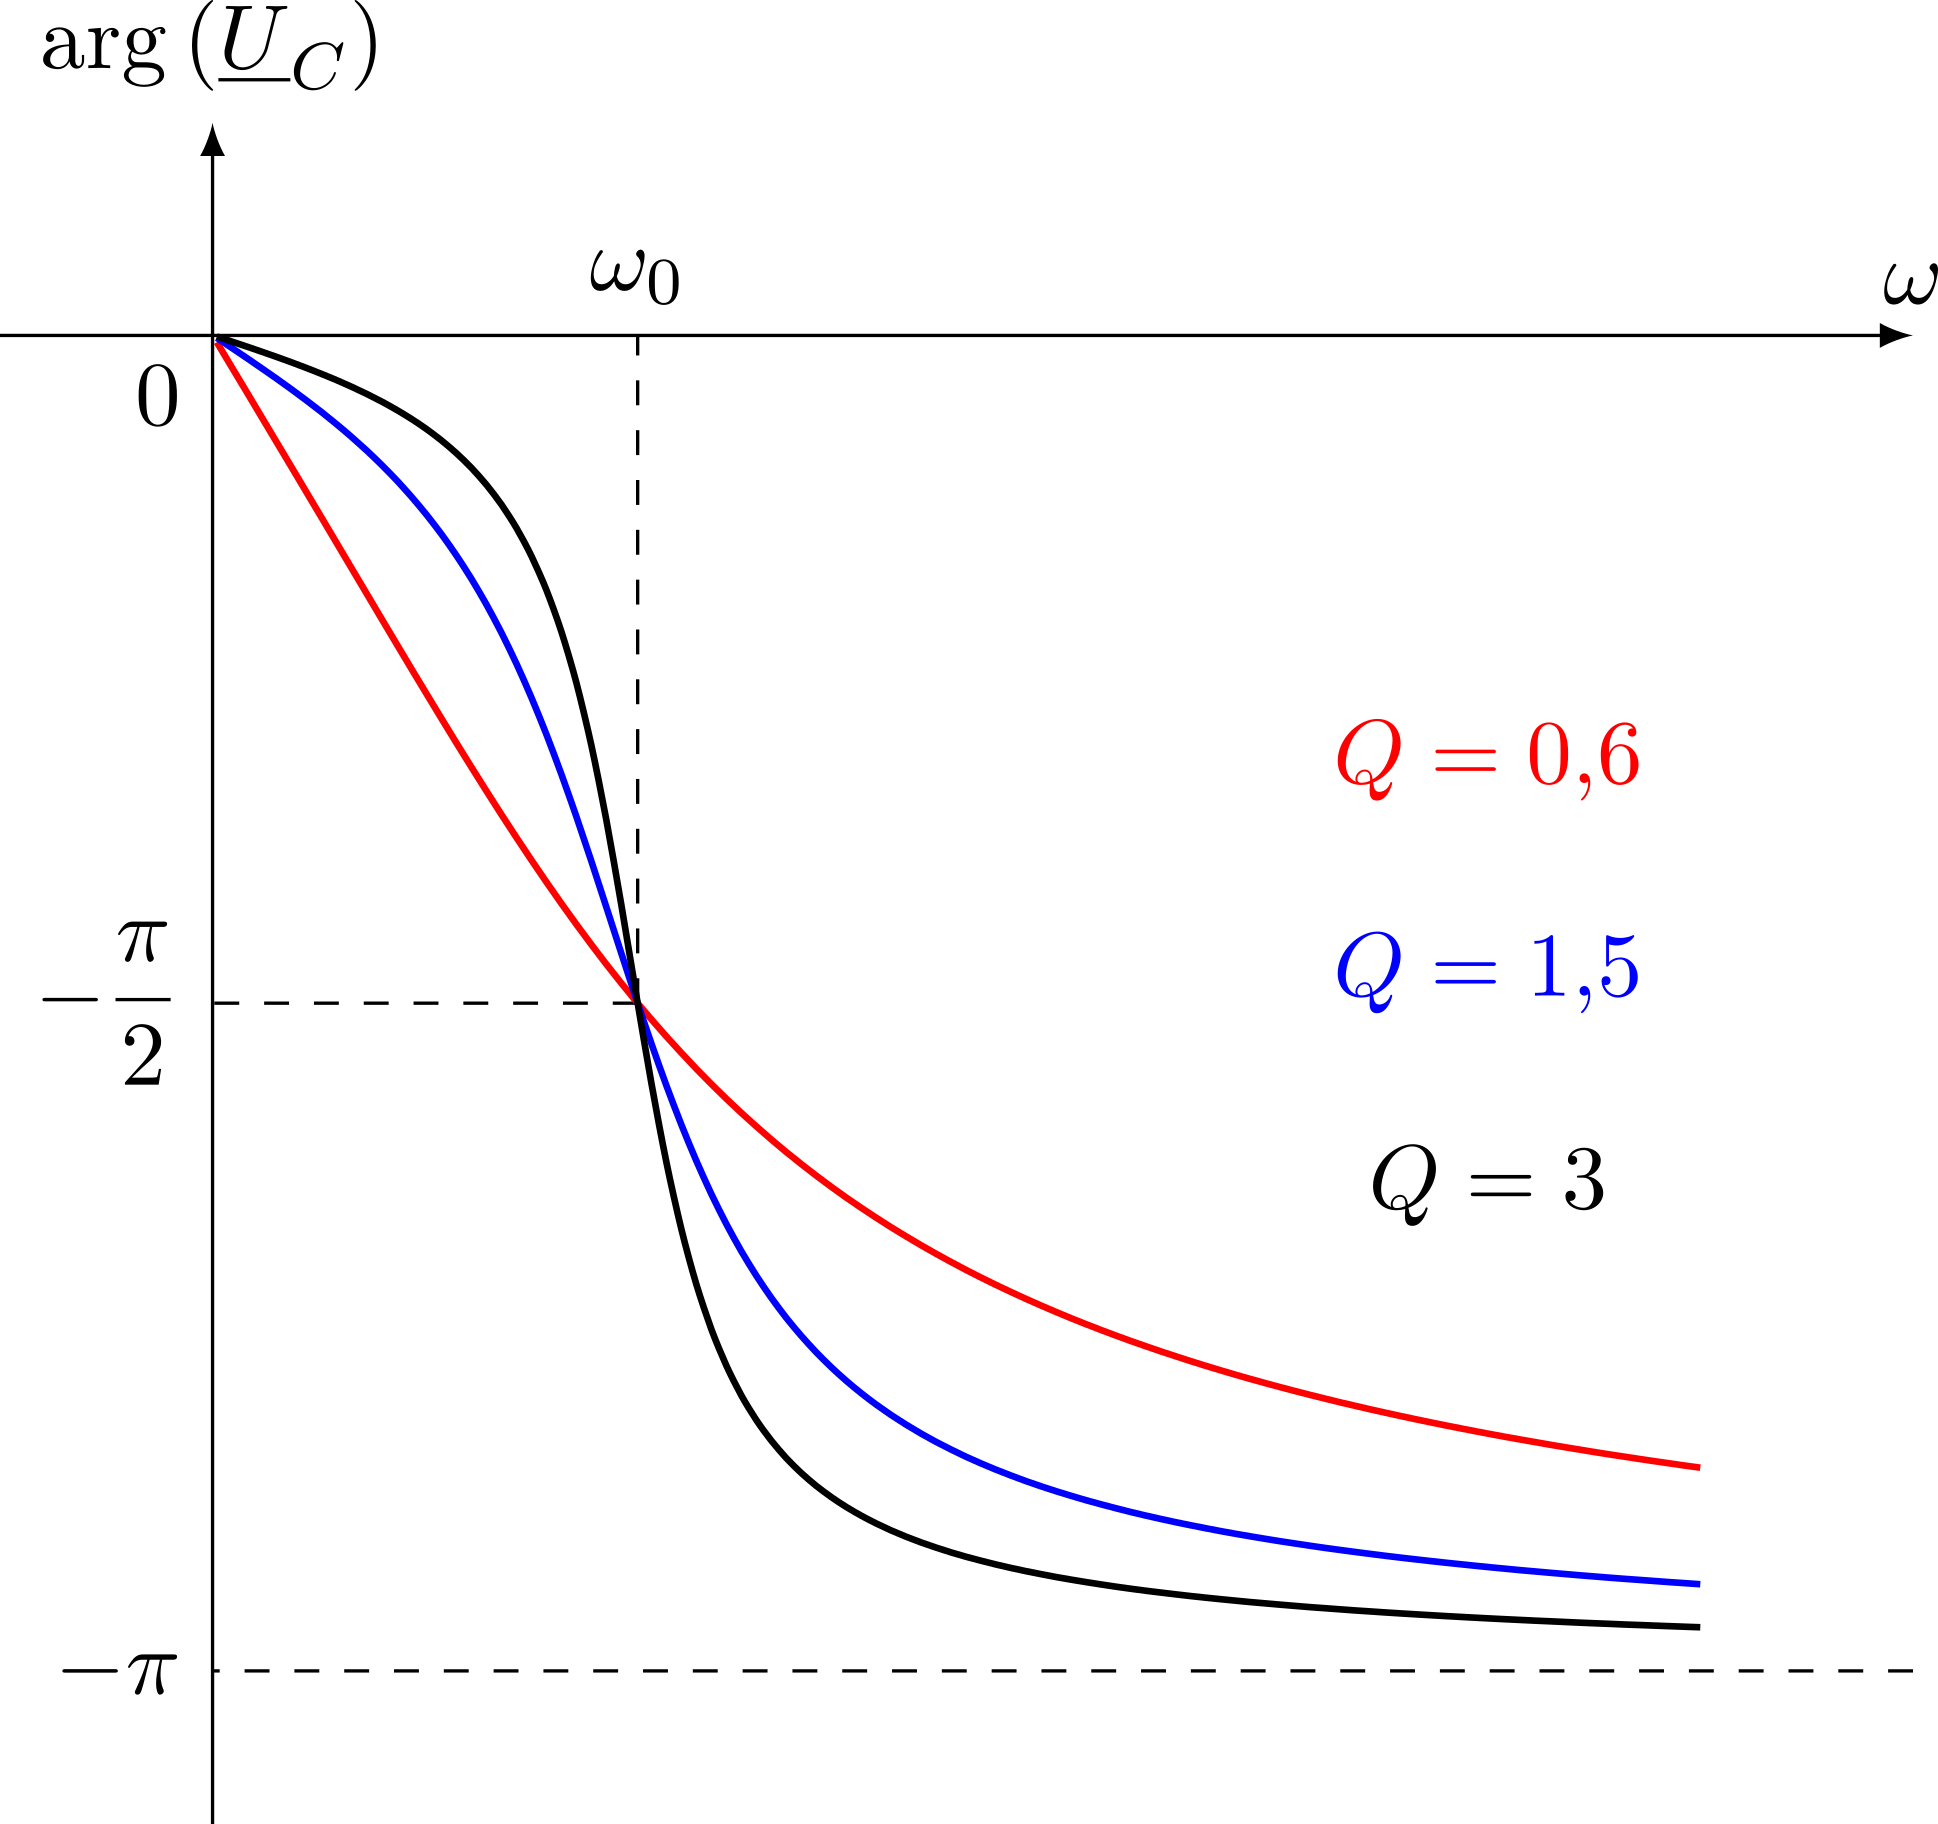
\includegraphics[width=.6\linewidth, draft=true]{rlc_u-phase}
	}{
		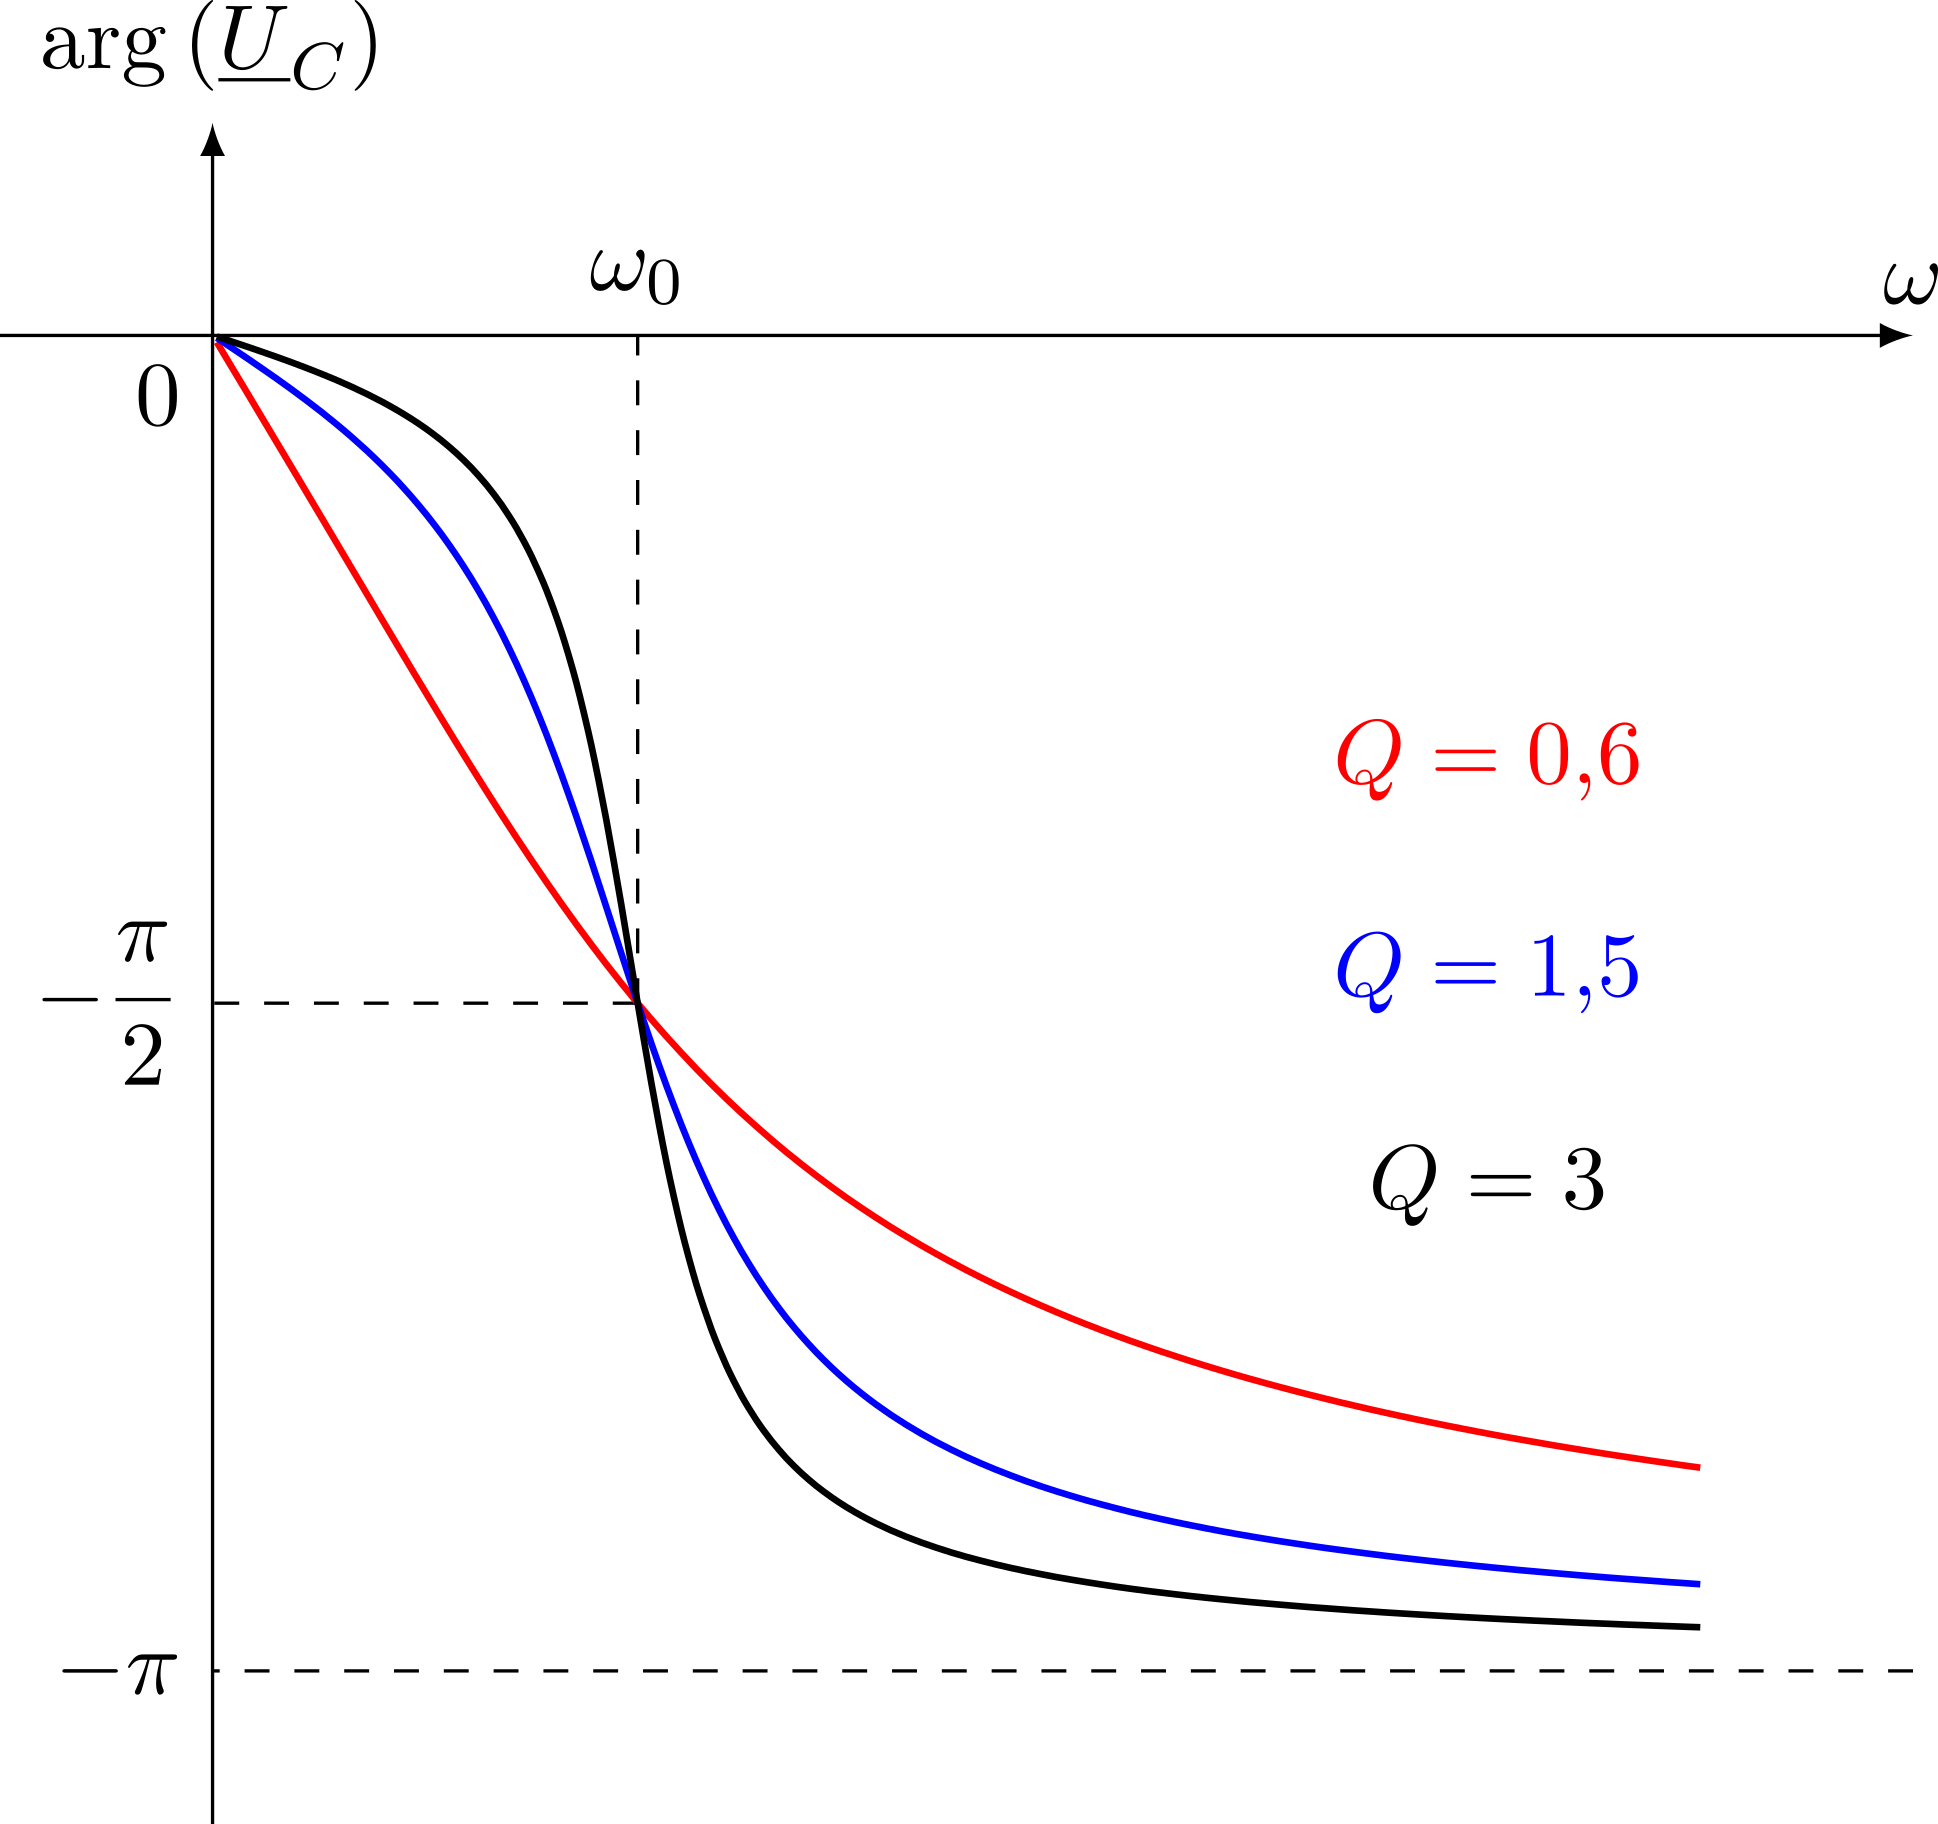
\includegraphics[width=.6\linewidth]{rlc_u-phase}
	}
\end{tcb}
\vspace{-15pt}
\end{document}
